\documentclass[]{article}\usepackage[]{graphicx}\usepackage[]{color}
%% maxwidth is the original width if it is less than linewidth
%% otherwise use linewidth (to make sure the graphics do not exceed the margin)
\makeatletter
\def\maxwidth{ %
  \ifdim\Gin@nat@width>\linewidth
    \linewidth
  \else
    \Gin@nat@width
  \fi
}
\makeatother

\definecolor{fgcolor}{rgb}{0.345, 0.345, 0.345}
\newcommand{\hlnum}[1]{\textcolor[rgb]{0.686,0.059,0.569}{#1}}%
\newcommand{\hlstr}[1]{\textcolor[rgb]{0.192,0.494,0.8}{#1}}%
\newcommand{\hlcom}[1]{\textcolor[rgb]{0.678,0.584,0.686}{\textit{#1}}}%
\newcommand{\hlopt}[1]{\textcolor[rgb]{0,0,0}{#1}}%
\newcommand{\hlstd}[1]{\textcolor[rgb]{0.345,0.345,0.345}{#1}}%
\newcommand{\hlkwa}[1]{\textcolor[rgb]{0.161,0.373,0.58}{\textbf{#1}}}%
\newcommand{\hlkwb}[1]{\textcolor[rgb]{0.69,0.353,0.396}{#1}}%
\newcommand{\hlkwc}[1]{\textcolor[rgb]{0.333,0.667,0.333}{#1}}%
\newcommand{\hlkwd}[1]{\textcolor[rgb]{0.737,0.353,0.396}{\textbf{#1}}}%

\usepackage{framed}
\makeatletter
\newenvironment{kframe}{%
 \def\at@end@of@kframe{}%
 \ifinner\ifhmode%
  \def\at@end@of@kframe{\end{minipage}}%
  \begin{minipage}{\columnwidth}%
 \fi\fi%
 \def\FrameCommand##1{\hskip\@totalleftmargin \hskip-\fboxsep
 \colorbox{shadecolor}{##1}\hskip-\fboxsep
     % There is no \\@totalrightmargin, so:
     \hskip-\linewidth \hskip-\@totalleftmargin \hskip\columnwidth}%
 \MakeFramed {\advance\hsize-\width
   \@totalleftmargin\z@ \linewidth\hsize
   \@setminipage}}%
 {\par\unskip\endMakeFramed%
 \at@end@of@kframe}
\makeatother

\definecolor{shadecolor}{rgb}{.97, .97, .97}
\definecolor{messagecolor}{rgb}{0, 0, 0}
\definecolor{warningcolor}{rgb}{1, 0, 1}
\definecolor{errorcolor}{rgb}{1, 0, 0}
\newenvironment{knitrout}{}{} % an empty environment to be redefined in TeX

\usepackage{alltt}
\usepackage{fontspec}
\usepackage{graphicx}
\usepackage{float}
\usepackage[hidelinks]{hyperref} % For linking Github

% \usepackage[left=2.54cm, top=2.54cm, right=2.54cm, bottom=2.54cm]{geometry}
\usepackage[left=1.27cm, top=1.27cm, right=1.27cm, bottom=2.54cm]{geometry}

\usepackage{pbox}
\setmainfont[Scale=1.25]{Cambria}
\linespread{1.25}
%\setmainfont[Ligatures=TeX,Scale=0.95]{Linux Libertine O}
\usepackage{pdflscape}

\usepackage{setspace}
% \doublespacing % For double-spacing. (From setspace)

\usepackage[document]{ragged2e} % For left-alignment.
\usepackage{parskip} % For space between paragraphs

% latexmk -pdf -pdflatex="xelatex -interaction=batchmode" -use-make -quiet tmle.tex

% If you use Biber, then you will have to compile and recompile.
% But Biber seems to be the preferred choice.
\usepackage[backend=biber,sorting=none,style=numeric-comp]{biblatex} 

\addbibresource{tmle.bib} % Critical that you put .bib in here!
\IfFileExists{upquote.sty}{\usepackage{upquote}}{}
\begin{document}
\title{Hospital readmissions and targeted maximum likelihood estimation}
\author{Aman Verma}
\date{\today}
% \maketitle

\begin{abstract}






Background: Hospitals in the US and other jurisdictions are being financially penalized based on estimates of their effect on 30-day readmission risk, after adjustment for confounders. Although hospital administrative data is information-rich, confounder adjustment in these models tends to be crude, risking residual confounding. Non-parametric machine learning techniques can take advantage of these rich data to predict readmission, but cannot isolate the independent effect of hospitals on readmission risk.

Research Design: To estimate the marginal effect of care at different hospitals on 30-day readmission risk, we used targeted maximum likelihood estimation (TMLE), which allowed us to use a non-parametric machine learning technique (random forest) to take advantage of the rich confounder data. We used an 11-year cohort of 65 year old patients from 20 hospitals in Montreal, Canada, and developed three models to estimate marginal readmission risk at each of the hospitals after hospitalization for heart failure, acute myocardial infarction (AMI), and pneumonia. To control for confounding, we modeled the effect of hundreds of types of pre-admission outpatient drug prescriptions, medical procedures, and diagnoses on readmission risk.

Results: Within 30 days of discharge, there were 5,520 / 24,847 (22\%) heart failure readmissions, 3,183 / 20,421 (16\%) pneumonia readmissions, and 2,525 / 15,746 (16\%) AMI readmissions. Within each hospital, there was a wide variation in crude readmission risk across the twenty hospitals for pneumonia 3,183 / 20,421 (16\%), heart failure 5,520 / 24,847 (22\%), and AMI 2,525 / 15,746 (16\%). However, after control for confounding, the marginal risk for readmission within all hospitals was nearly the same (within each admission category).

Conclusion: Although crude readmission risk estimates between hospitals may show wide variation, there may be little difference in marginal risks after control for confounding.

\end{abstract}

\section{Introduction}
% Why is this question important to answer?
% I refuse to put in that horrible estimate of the cost of readmissions.
In the early eighties, hospital administrators in the US sought to reduce hospitalization costs by changing the reimbursement system. Instead of paying hospitals per day of hospitalization, hospitals were paid a fixed rate for the type of hospitalization and the procedures performed. Following implementation of this law, the length of stay at hospitals dropped dramatically, although evidence exists that is was already in decline. 

% Bring in the AMI, pneumonia, heart failure here somewhere.
Some worry that the new system created a perverse incentive to discharge patients early, and admit them again at a later date. To ensure proper quality of care in the hospitals while keeping costs controlled, administrators have sought to establish useful quality of care metrics. Hospital readmissions have been identified as a simple metric that can establish a baseline of care; if an abnormally high number of patients from a certain hospital are quickly readmitted, it could indicate poor quality of care. 

%  So, our main problem is confounding.
Since hospitals admit patients with varying risk of readmission, it is important to accurately estimate the effect of hospital treatment on readmission independent of patient-level confounders. Without effectively controlling for confounding, we risk unfairly penalizing hospitals that treat sicker (more likely to be readmitted) patients. Fortunately, hospital and outpatient administrative data is information-rich. Drug prescriptions, diagnoses, and medical procedures can provide important information on how the effect of hospital care on readmission risk is confounded by patient health. 

% How do studies typically control for confounding?
However, in most statistical models of readmission risk, the hospital administrative data is simplified to a few well-known confounders (age, sex, previous readmissions), and sometimes a summary "comorbidity score". If each drug, diagnosis and procedure was modeled with a separate covariate, the model would be very computationally expensive to fit. Such a model would also be very unwieldy to develop; analyzing how inclusion or exclusion of variables affects the model would be impossible to do effectively with hundreds of covariates. 

% Why is that problematic?
By summarizing confounders into crude risk scores, we risk "residual confounding" leading to biased effect estimates. Furthermore, to compare hospitals, we are only interested in estimating one parameter, the independent effect of hospitals on readmissions. We are only interested in the other variables insofar as they confound the effect of hospitals on readmissions, estimating the individual effect of each of these variables is unnecessary, and statistically wasteful.

% We can use machine learning techniques to develop a model with thousands of covariates.
Non-parametric machine learning techniques are available that will let us accurately discriminate patient readmission risk using hundreds of variables in a computationally efficient way. Furthermore, because they are non-parametric, we avoid having to specify a functional form, and can find complex "interactions" between variables. On the other hand, these non-parametric techniques don't allow us to isolate (target) the effect of specific variables (such as care at a particular hospital) on readmission risk. 

% Instead of summarizing comorbidity scores using expert knowledge, we use the data to develop a comorbidity score specific to the problem at hand.

The targeted maximum likelihood estimator (TMLE), is a doubly-robust technique that uses propensity scores to estimate target parameters of interest from non-parametric (or parametric) models. To use TMLE, a model is developed to estimate the probability of exposure (the propensity score), and also fit another model to estimate the probability of outcome. These two probabilities are combined in a parametric model with only the parameter of interest, inversely weighted by the probability of exposure, and offset by the probability of the outcome. In this way, the discriminative power of non-parametric models can be used to extract estimates of parameters of interest. 

% What is the study question?
In this study, we sought to estimate the marginal risk of readmission within 30 days of discharge for three different admission diagnoses (pneumonia, heart failure, and acute myocardial infarction) for each of twenty Montreal hospitals. We used a ten-year cohort of 65 year old people, for which we had outpatient and inpatient diagnoses  and procedures, and outpatient drugs prescriptions. We used a non-parametric machine learning technique, (random forest), with TMLE to take advantage of the rich confounder data and provide less biased estimates of readmission risk at each hospital. 

% To estimate propensity of attending different hospitals as a function of hundreds of covariates relating to patient health, we used a non-parametric machine learning technique, random forest. We combined this propensity with a more traditional model of hospital readmissions as a function of hospital care and patient characteristics (penalized logistic regression) with a doubly robust technique, targeted maximum likelihood estimation (TMLE).
\section{Methods}

\subsection{Data}
% What does our cohort look like?

\subsubsection{Cohort selection}
We used a cohort extracted from a Canadian provincial (Quebec) administrative database of hospitalizations, obtained from the \emph{Régie de l'assurance maladie du Québec} (RAMQ). We enrolled patients into this cohort on the month that two conditions were satisfied: 1) they had at least one diagnosis of a respiratory illness (the exact list of respiratory International Classification of Diseases, 9th Revision [ICD-9] codes is given in the Appendix) between January 1st, 1996 and March 31, 2006 (the study period), while living in the 2006 census metropolitan area of Montreal, and 2) were at least 65 years of age. We used this cohort because it represents the majority of 65-year olds who were hospitalized in the region during the study period. 

From among this cohort, we selected hospital discharges for those who had accrued at least one continuous year in the cohort preceding the time of admission. We restricted our data to only the discharges from the twenty hospitals with the most discharges of patients 65 years or older within the study period; the twenty hospitals accounted for 75\% of all such discharges.  We only selected hospital discharges which resulted from hospital stays of at least one day. Therefore, the earliest possible hospital discharge was January 2, 1997.

\subsubsection{Hospital readmissions}
The unit of analysis was the hospital discharge; a person could be discharged multiple times. A hospital readmission was defined as an emergency hospital admission to any Quebec hospital in the 30 days following a discharge.  A person who died or had a non-emergency readmission in the 30 days following discharge was considered not readmitted.

\subsubsection{Disease types}
From among the identified hospital discharges, we selected only those with one of three high-volume admission diagnoses with high rates of hospital readmissions: pneumonia, acute myocardial infarction (AMI), and heart failure, the three initial conditions selected by the Centers for Medicare and Medicaid Services (CMS) to implement the Hospital Readmissions Reduction Program mandated by the Affordable Care Act. We identified each of the admission diagnoses using ICD-9 codes; for pneumonia we used codes ranging from 480-487, for heart failure we used all 428 codes, and for AMI we used all 410 codes. The following methods were applied individually to all three disease subsets. 

% Should I talk about the anonymization of hospitals?

% We had confounders.
\subsection{Confounders}
% The basic demographics and time-related confounders.
For each hospital discharge, we colllected variables that measured states at the time of admission, or events that occurred prior to the hospital admission, and which may confound the relationship between hospital care and readmission. We used the demographic characteristics (age at time of admission (years), sex, birth year-month), the number of previous readmissions (within the preceding year), the admission diagnosis (as measured by the specific ICD-9 code). We also included the day of week of discharge, which has been previously shown to have an association with readmissions\supercite{}, and the month of discharge, because we hypothesized that readmission risk would vary by seasons in Montreal.

% Procedures, drugs, and diagnoses.
Additionally, for each discharge, we collected the Quebec hospital diagnoses, Quebec hospital procedures, and drugs dispensed outside of the hospital but inside Quebec, in the year preceding the admission. The hospital procedures were recorded in the Canadian Classification of Diagnostic, Therapeutic, and Surgical Procedures (CCP) system. Hospital diagnostic codes were coded using the ICD-9 system. Finally, drugs which were prescribed and dispensed outside the hospital, and were being taken on the day of admission were also recorded for each patient in the \emph{code commune} system, which categorizes drugs based on the chemical compound. To ease computation, before fitting any model, we removed any diagnosis, procedure or drug that occurred less than 30 times among all discharges. We chose 30 because it appeared to be a natural breakpoint; if the number of variables included is a function $f$ of the threshold, then the first derivative of $f$ dropped at 30 for all three disease categories.

% Area of residence.
We believed that residential location would strongly affect the probability of admission to the hospital nearest that census tract. We included it in our models because we also expected it to crudely approximate a (expected) confounder: socio-economic status.  We used the residential postal code at the time of admission to assign each patient in the cohort to a census tract, as defined by the 2006 Canadian census. (Census tracts contain between 2,500 and 8,000 people, and, at the time of their creation, are demarcated so as to maximize homogeneity of socioeconomic characteristics.)

\section{Modeling with targeted maximum likelihood estimation}
To esimate the marginal risk of 30-day readmission for each of the twenty hospitals, we used targeted maximum likelihood estimation. The process consisted of three steps 1) estimation of a propensity score ($g$), 2) an initial estimate of the risk of readmission based on all confounders and the variables for each of the hospitals ($Q$), and 3) a final step in which we fit twenty models ($Q*$), in which a single parameter was fit to the inverse probability of exposure to that hospital (as estimated by $g$), and each offset by the marginal readmission risk of attending that hospital (as estimated by $Q$). 

\subsection{Random forest}
To estimate both models $g$ and $Q$, we used a random forest, a non-parametric model based on decision trees \supercite{breiman_random_2001}. Decision trees repeatedly split data into partitions that are as homogenous as possible with respect to the outcome of interest. Complex interactions and non-linearities are naturally modeled within this framework. Random forest improves decision trees by using bootstrap aggregation (bagging); multiple decision trees are grown on bootstrap replicates (sampled with replacement) to avoid overfitting. Additionally, within each tree, only a sample of the covariates is used (in our case we used a square root of the number of variables, rounded down, included in the model).

For both $Q$ and $g$, we arbitrarily chose to grow 1200 trees, and then measured the accuracy as a function of the number of trees to ensure that growing further trees would be unlikely to significantly improve accuracy. When measuring the accuracy for each discharge, we only used trees for which the discharge was "out-of-bag", that is, we only used trees for which the bootstrap sample did not include the discharge.

\subsubsection{Model $g$ - probability of exposure}
% We built a model G
Using random forest, we developed a multinomial model $g$ that predicted the probability of attending each of the twenty hospitals (a propensity score) as a function of all the measured confounders. 

Random forest traditionally classifies each item by majority vote; we converted this into a probability by taking the proportion of votes for each hospital (using only out-of-bag trees for each discharge).


% How the Gini coefficient works.
% Make it clear that you didn't invent this.
To assess the importance of the variables in predicting which hospital a patient will choose, for each tree, we calculate the increase in homogeneity of classes between the root of the tree and the leaves. To measure the homogeneity of classes, we repurpose a metric that is typically used to measure equality (homogeneity) of income, the Gini coefficient \supercite{gini_variabilita_1912}. The homogeneity is defined as the sum of squared proportions in each class (hospital), with a maximum of 1 (all discharges at the same hospital) and a minimum of 1/20 (the discharges were evenly divided between the 20 hospitals). If the patients within the leaves of the tree made relatively homogeneous hospital choices, this variable predicts hospital choice well.

% We calibrated it based on the weights of the hospital. It was multinomial in that we predicted 20 hospitals. We measured the calibration, similarly only using out-of-bag discharges. We investigated the top 10 varibales most important variables, as measured by the Gini coefficient. 
 
% How we weighted -- still haven't put in how it was the *Gini* that was weighted.
Because the model was used solely to estimate the \emph{probability} of admission to to specific hospitals (and not to predict exactly which hospital was attended), we configured the model to favour calibration over discrimination: we weighted each of the twenty predicted hospitals by the inverse of the proportion of discharges at that hospital. We multiplied each proportion used to calculate the Gini coefficient by this weight.


\subsubsection{\(Q\) model - probability of outcome}
% We built a model Q
% We built another random forest model, very similar to the model for G, except that instead of predicting the choice of hospital, we predicted 30-day readmission. We also included a set of 19 indicator variables (or was it twenty?) for the hospital. This was also calibrated based on the inverse of the proportion of those readmitted.
For the  \(Q\) model, we developed another random forest model, very similar to the \(g\) model, except that instead of predicting the choice of hospital, we directly predicted 30-day readmission. We also included a set of 20 indicator variables for the hospital attended. We also calibrated this model based on the inverse of the proportion of those readmitted.

We also fit a regularized logistic regression model for \(Q\), using cyclical coordinate descent to estimate the parameters efficiently in our sparse but large information matrix. We penalized the likelihood by the \(\ell_2\) norm, that is, the sum of the squares of the normalized regression parameters. The scale of the penalty was determined by the parameter λ. We optimized the selection of the penalty scale for the best partial likelihood using a nested a 10-fold cross-validation. Within each fold we assessed 100 λ-values spaced evenly between max(λ)×10-4 and max(λ), where max(λ) was the smallest λ-value that would result in a model with no non-zero coefficients.

\subsubsection{Variable importance}
% What is the ref for the Gini coefficient?
For each tree, we calculated the decrease in Gini homogeneity when comparing the split nodes of the tree to the root. 
The Gini impurity at any node is, for all out-of-bag discharges.

% To calculate the Gini impurity..
For each hospital, the proportion of patients that chose this hospital $p_h$, multiplied by the probability of guessing that this patient would choose this hospital based on the distribution of patients $1-p_h$. Summed over all hospitals, this is the Gini impurity. Gini impurity is 1 when all patients chose the same hospital.

Gini is defined as "inequity" when used in describing a society's distribution of income, or a measure of "node impurity" in tree-based classification. A low Gini (i.e. higher decrease in Gini) means that a particular predictor variable plays a greater role in partitioning the data into the defined classes. 


\subsubsection{Model Q* - updated targeted maximum likelihood estimation}
To combine our both our models G and Q, we fit twenty (one for each hospital) one-parameter logistic regression models called Q*. Q* was fit as a logistic regression with no intercept; we regressed readmission on to the inverse probability of exposure to that hospital, offset by the Q's prediction of readmission. We then used Q* to calculate the marginal probability of exposure for each hospital.

% We updated for Q*
To avoid convergence problems for this one parameter model, we fit the parameter using a quasi-Newton method simultaneously discovered by Broyden\supercite{broyden_convergence_1970}, Fletcher\supercite{fletcher_new_1970}, Goldfarb\supercite{goldfarb_family_1970} and Shanno\supercite{shanno_conditioning_1970} (BFGS).

\subsection{Time-to-event analysis}
% As described in Stitleman.
We also modeled the time-to-readmission as a function of the hospital the patient receieved care at. Thirty days is an arbitrary cutoff, time-to-event allows us to differentiate between more nuanced differences in readmission times.

In general, we followed the method for (non-collaborative) TMLE for survival analysis outlined in Stitleman, with a few deviations. The survival analysis required a model of the exposure as a function of the covariates; we resued the random forest model for $g$ as outlined above.

In addition, we needed to develop models that estimated the survival function of both readmission (model $Q$), and right-censoring (model $g_2$). (The survival function $S(t)$ is the probability that a random person selected from the cohort has a probability of readmission [censoring] is greater than $t$.) A person was considered right-censored if they died, had a non-emergency readmission, they changed residence to a location outside of Quebec, or the study ended. 

We estimated both survival functions in two steps, we first fit a Cox proportional hazards model, and then used that model to estimate a baseline survival function.  We fit a regularized Cox proportional hazards model for both \(Q\) and \(g_2\), using cyclical coordinate descent to estimate the parameters efficiently in our sparse but large information matrix. We penalized the likelihood by the \(\ell_2\) norm, also known as the lasso penalty. The scale of the penalty was determined by the parameter λ. We optimized the selection of the penalty scale for the best partial likelihood using a nested a 10-fold cross-validation. Within each fold we assessed 100 λ-values spaced evenly between max(λ)×10-4 and max(λ), where max(λ) was the smallest λ-value that would result in a model with no non-zero coefficients.

We then estimated the baseline survival function using the technique described in Fleming and Harrington. We combined the baseline survival function with the individual-level covariates to get the covariate-level specific survival function for each individual. We calculated the twenty readmission survival curves for each person, one for each hospital. We also calculated twenty censoring survival curves.
% Fleming, T. H. and Harrington, D. P. (1984). Nonparametric estimation of the survival distribution in censored data. Comm. in Statistics 13, 2469-86. 

For each hospital, for each person-day, we computed the "clever covariate", which is a function of the readmission survival function, the censoring survival function, and the probability of hospital exposure. Using logistic regression (without an intercept term), we regressed the binary readmission status offset by the inverse logit of the conditional failure probability, at every unit of person-time, on to the clever covariate, yielding a single parameter epsilon. We then iterated the procedure: we repeated the same logistic regression, except that we offset the binary readmission status by the inverse logit of the conditional failure probability plus the epsilon in the previous iteration. We iterated until the epsilon was less than $1^-10$.

Using the sum of the epsilons for all iterations for each hospital, we could then compute an "updated" survival function for each person for each hospital, which allowed us to estimate the expected time-to-readmission for each person as if they were cared for at each separate hospital. We compared the distribution of marginal survival times, as well as the marginal mean and median survival times.

\subsection{Software}
The data were cleaned and prepared for statistical analysis using the Postgres relational database (version 9.2.6). We implemented our models using the R statistical package (version 3.1.0) \supercite{team_r:_2014}. We implemented the random forest using the "bigrf" package (version 0.1.11) \supercite{lim_bigrf:_2014}. We implemented the GLM fitting using coordinate descent using the "glmnet" package (version 1.9.8) \supercite{friedman_regularization_2010}. We plotted our figures using the "ggplot2" package (version 1.0.0) \supercite{wickham_ggplot2:_2009}. All the code to develop used to fit clean our data, fit our models, and layout this paper is \href{https://github.com/nograpes/tmle_readmissions}{available for download at Github}.

\section{Results}
% A pretty map for pretty much no reason. It shows that indeed, certain hospitals attract the residents around them, and that this does not vary by disease.

% We believed that census tract of residence would strongly affect the probability of admission to the hospital nearest that census tract. We plotted choropleths of the rate of attendance at the twenty hospitals by census tract. The numerator was the number of live discharges at the hospital, and the denominator was the number of person-years accumulated in that census tract of residence by cohort members when their admissions would have been eligible (after the first continuous year within the cohort).

% \begin{figure}[H]
%     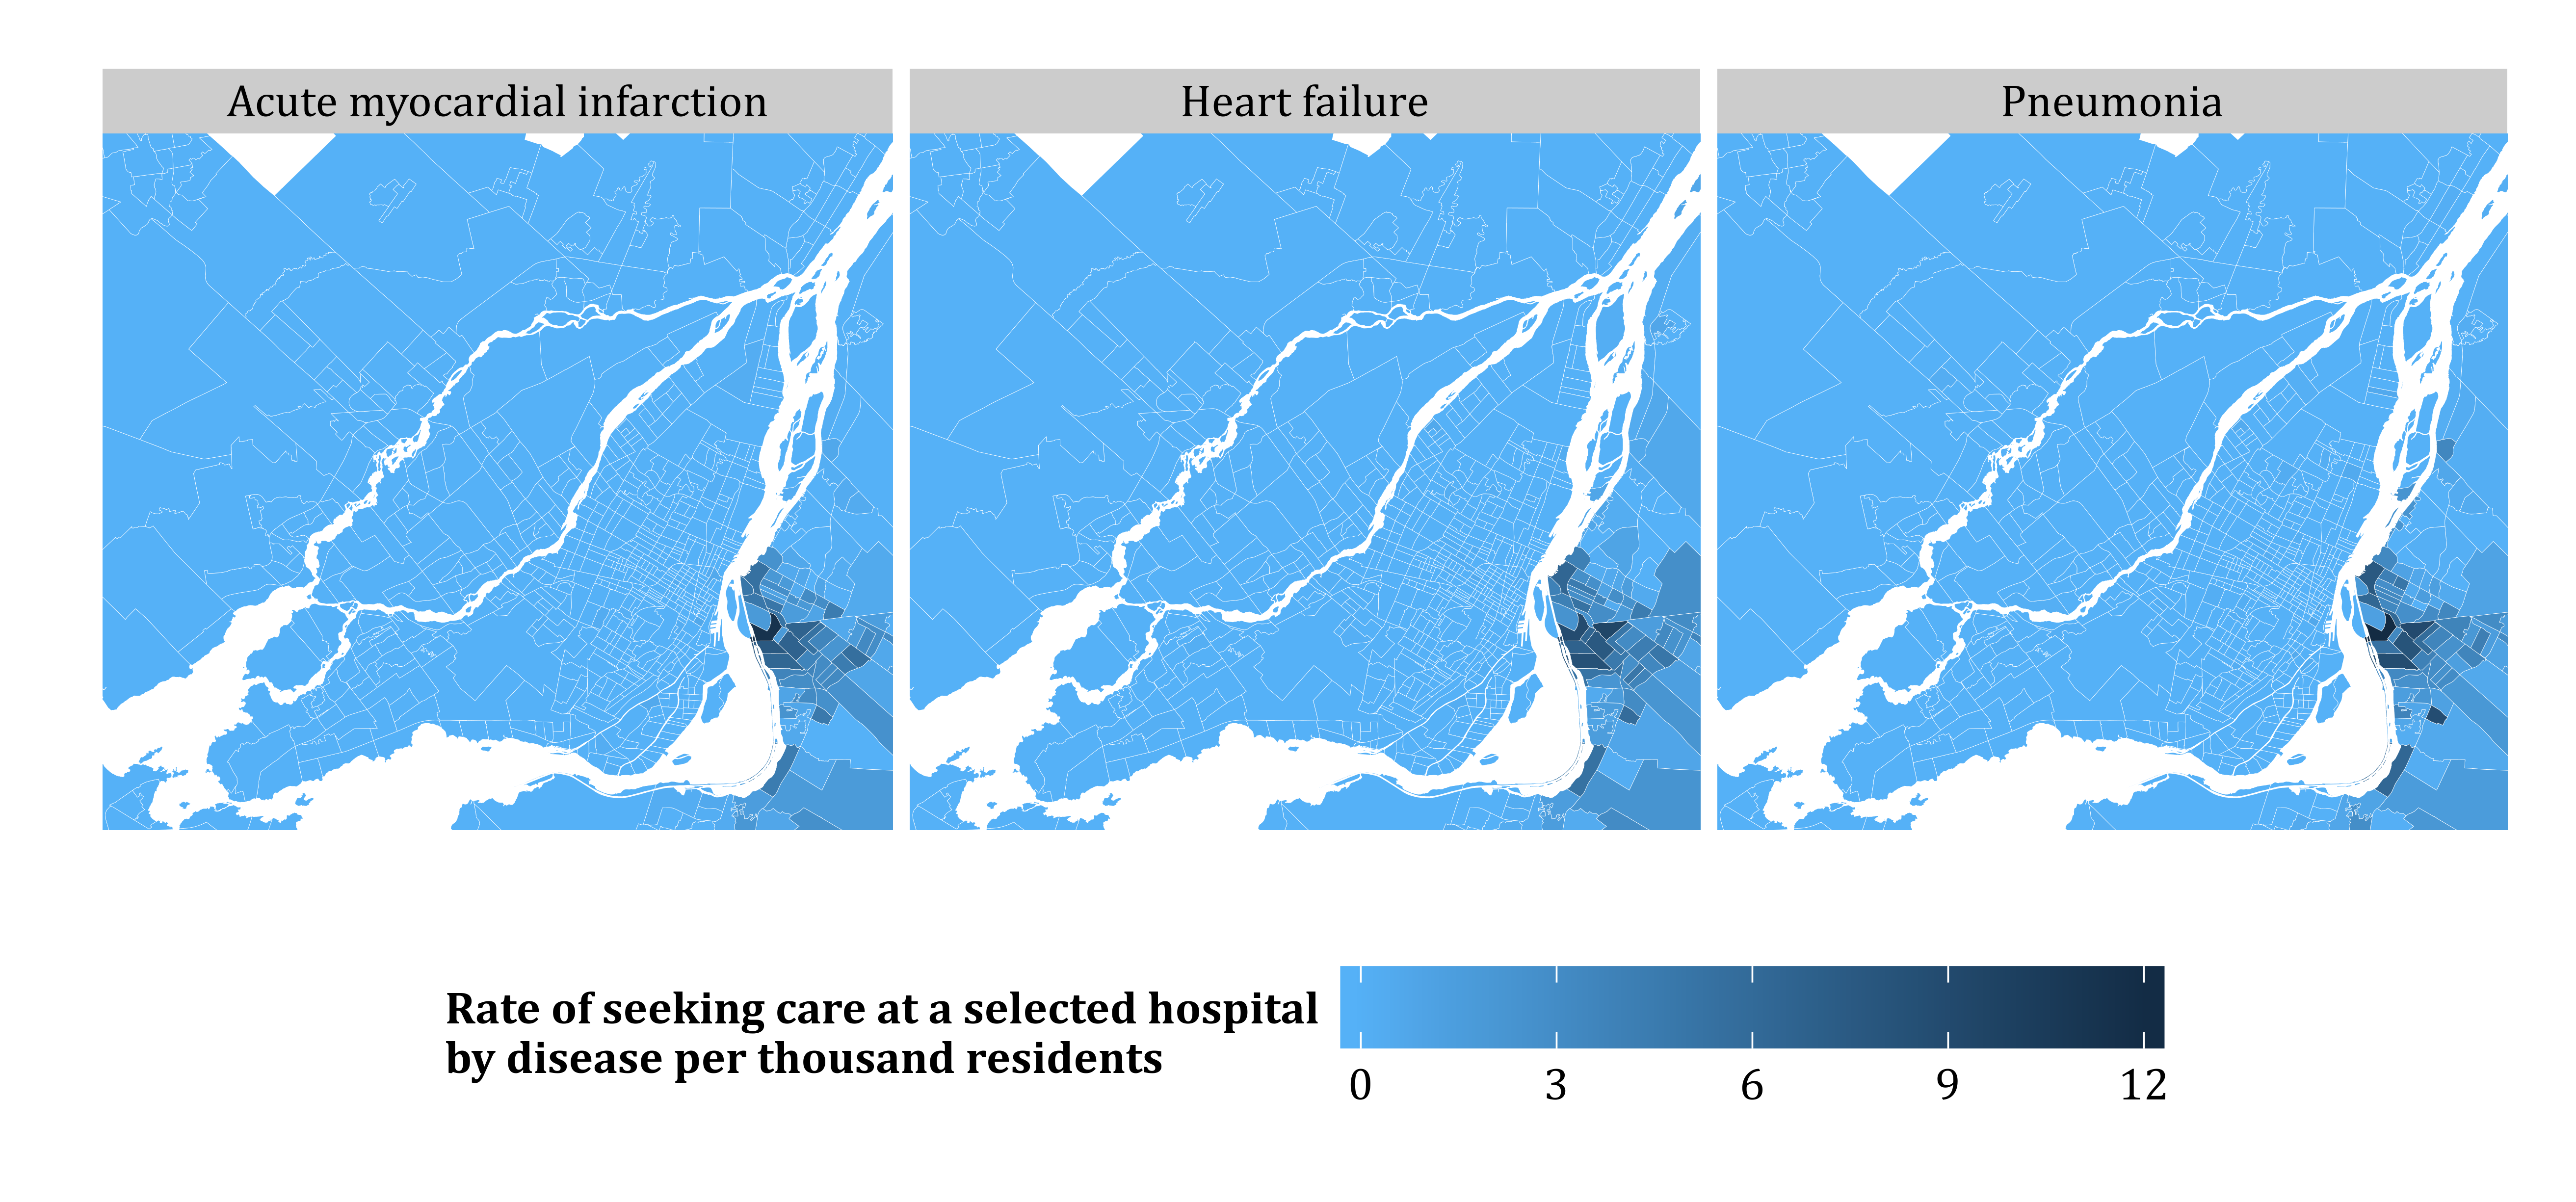
\includegraphics{../figures/hosp_choro.png}
%     \caption[Rates of seeking care at a selected hospital by admission diagnosis.]
% {Rates of seeking care at a selected hospital by admission diagnosis in the island of Montreal. The numerator was the number of live discharges at the hospital, and the denominator was the number of person-years accumulated in that census tract of residence by cohort members when their admissions would have been eligible (after the first continuous year within the cohort). The areal units are census tracts.}
%     \label{fig:hosp_choro}
% \end{figure}

Over the course of January 2, 1996 to March 31, 2006, 482 064 people were entered into our cohort. 

Among these, x were ever admitted for pneumonia, y were ever admitted for AMI, and z were ever admitted for heart failure. 

People ever admitted for pneumonia had a mean of x and median x2 pneumonia admissions , ever heart failure patients had a mean h1 and median h2 heart failure admissions, and ever AMI patients had a mean a1 and median a2 heart failure admissions.

% What does the accuracy of the random forest model look like as the number of trees grows for both the Q model and the G model?
\begin{figure}[H]
    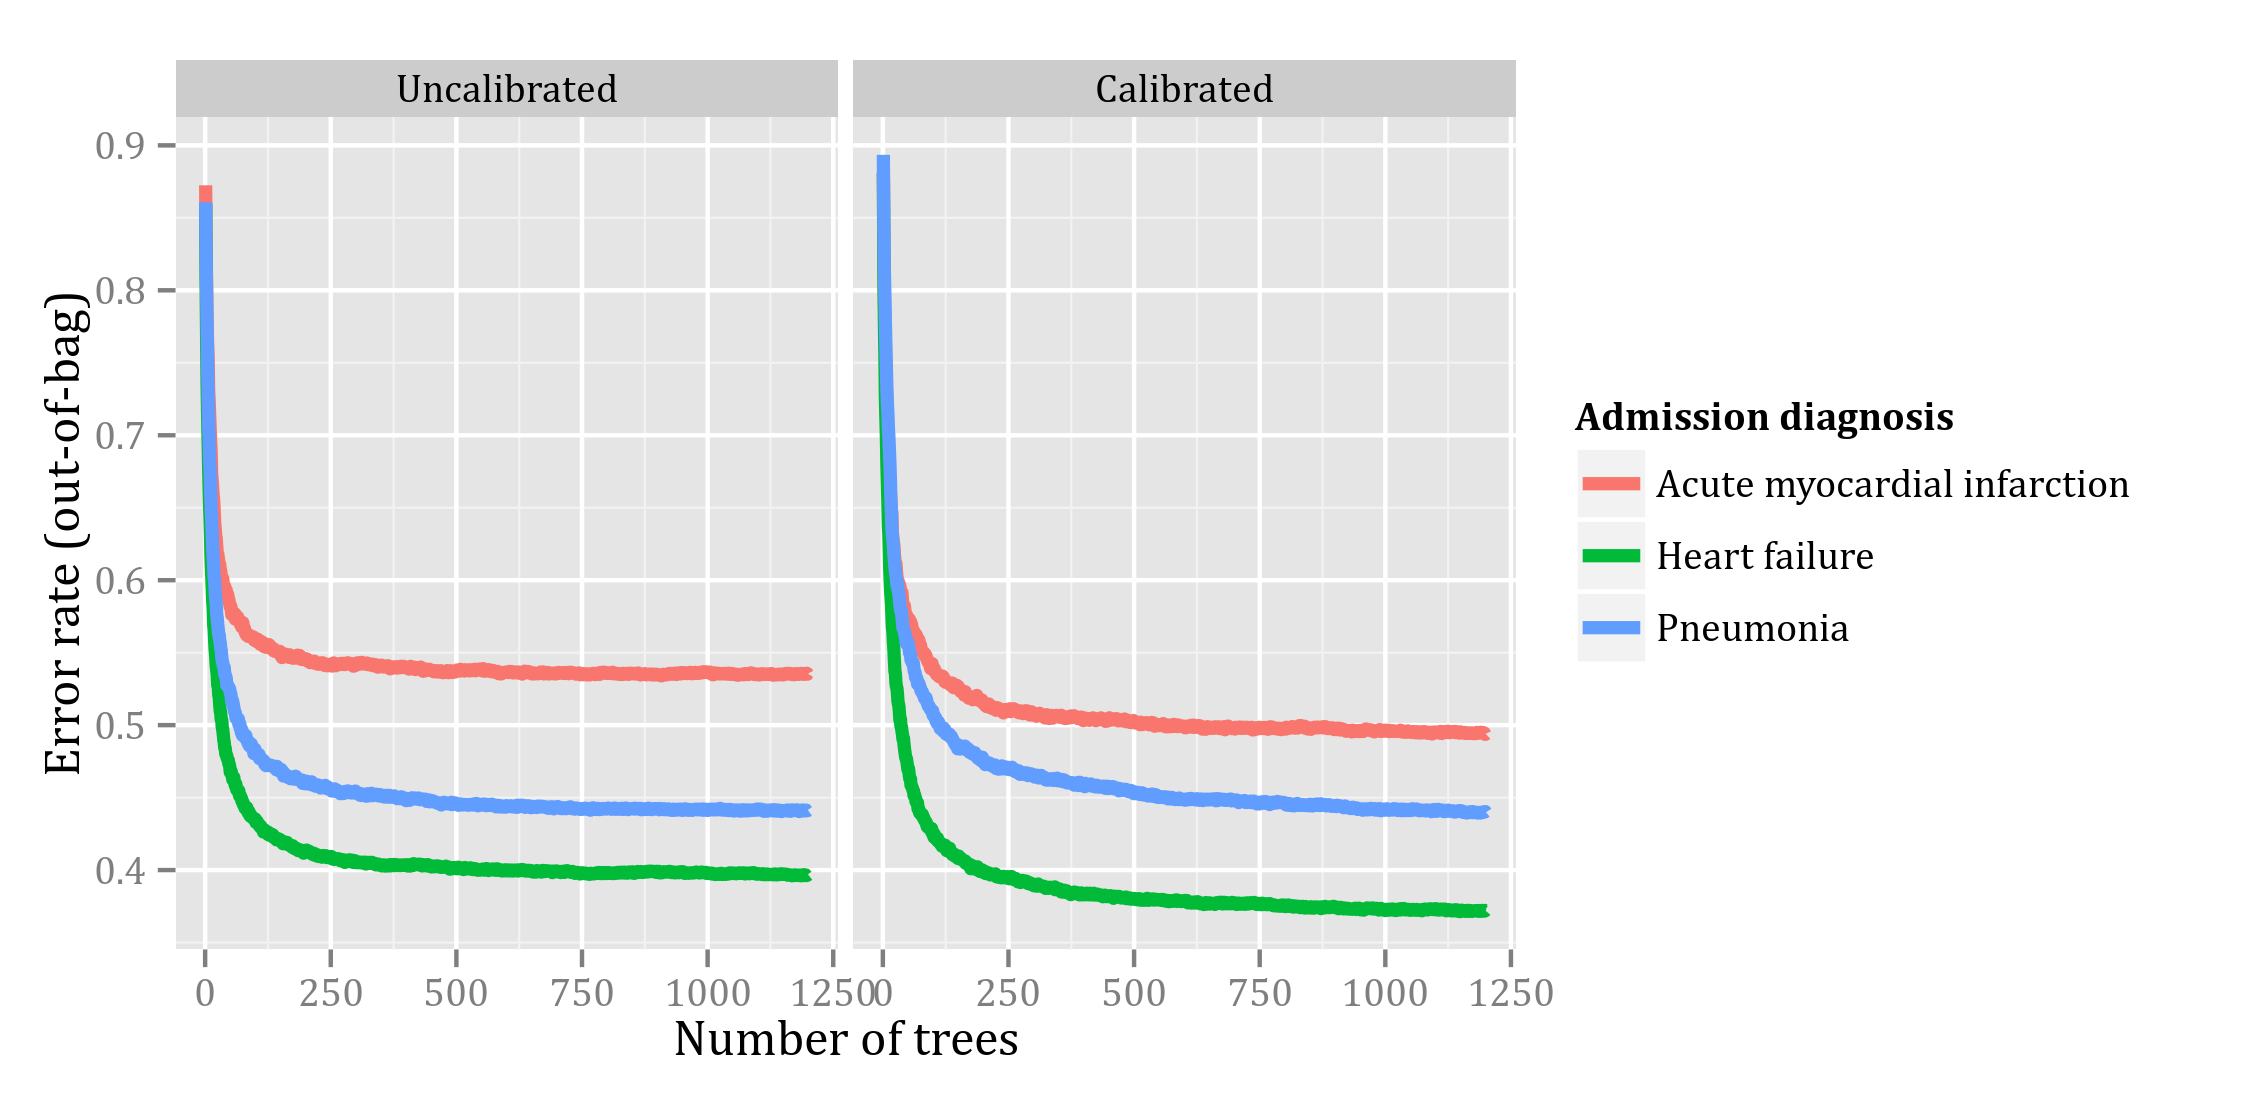
\includegraphics{../figures/error_rate_for_hospital_choice.png}
    \caption[Error rate for random forest model of hospital choice.]
      {Error rate for both random forest models of hospital choice (g) and readmission (Q) as a function of the number of trees grown. For each admission, only out-of-bag trees were used to predict the given outcome.}
    \label{fig:error_rate_for_hospital_choice}
\end{figure}

% Calibration of random forest
% \begin{figure}[H]
%     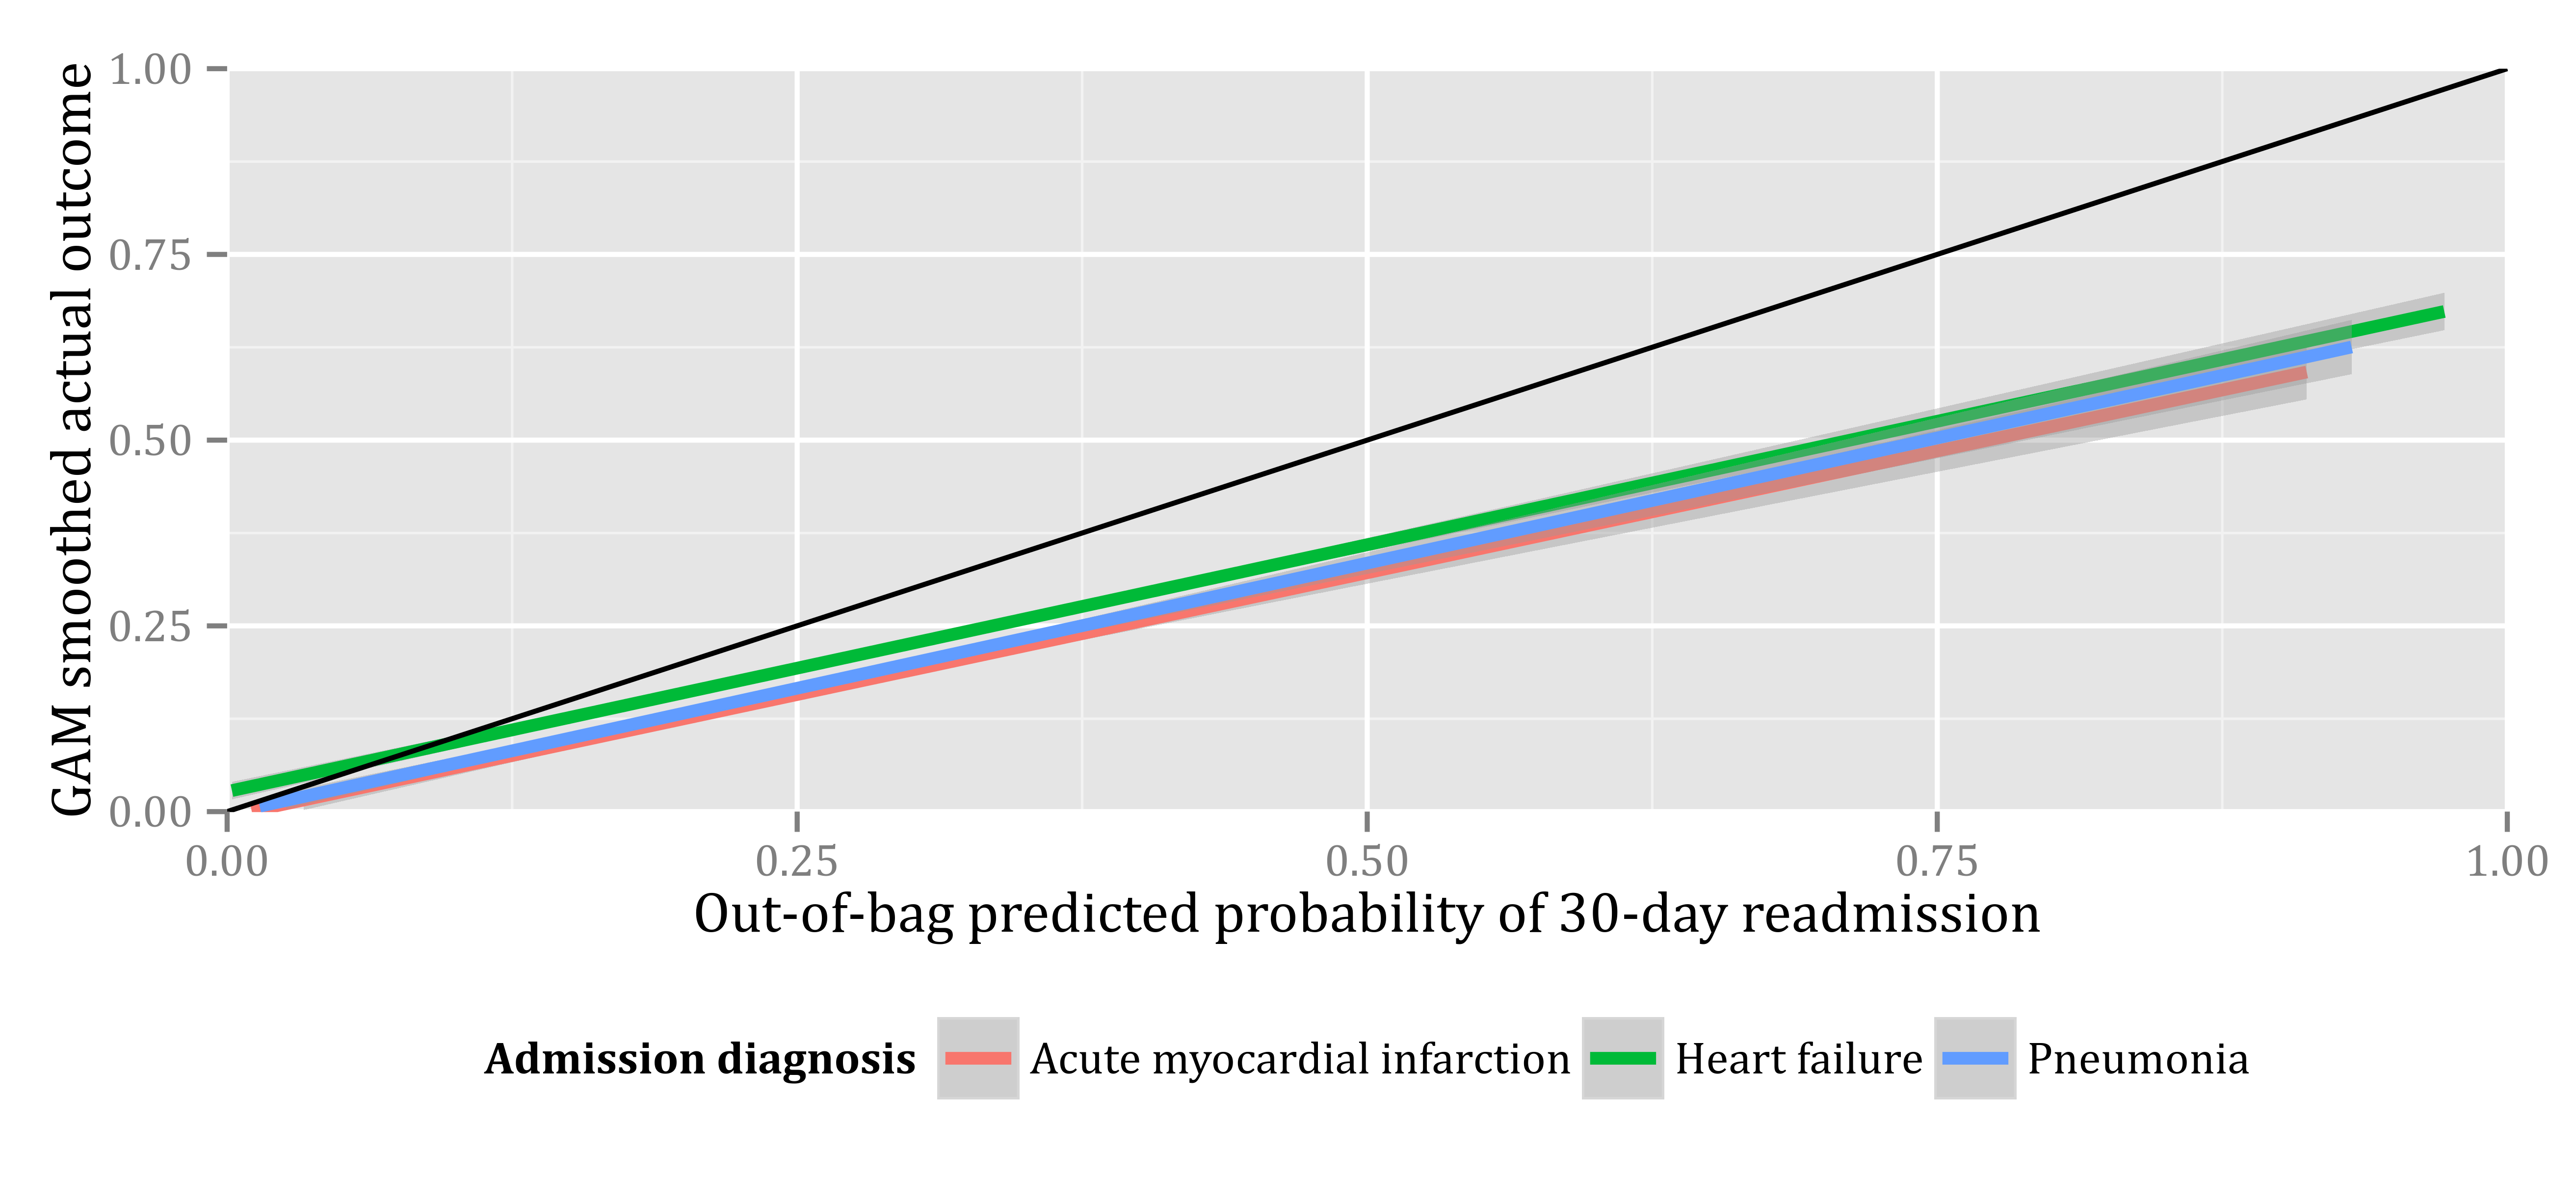
\includegraphics{../figures/rf_calibration.png}
%     \caption[Calibration for random forest model of hospital readmission.]
%       {Calibration for random forest model of hospital readmission. A descriptive sentence.}
%     \label{fig:error_rate_for_hospital_choice}
% \end{figure}
% 
% % Calibration of GLMnet
% \begin{figure}[H]
%     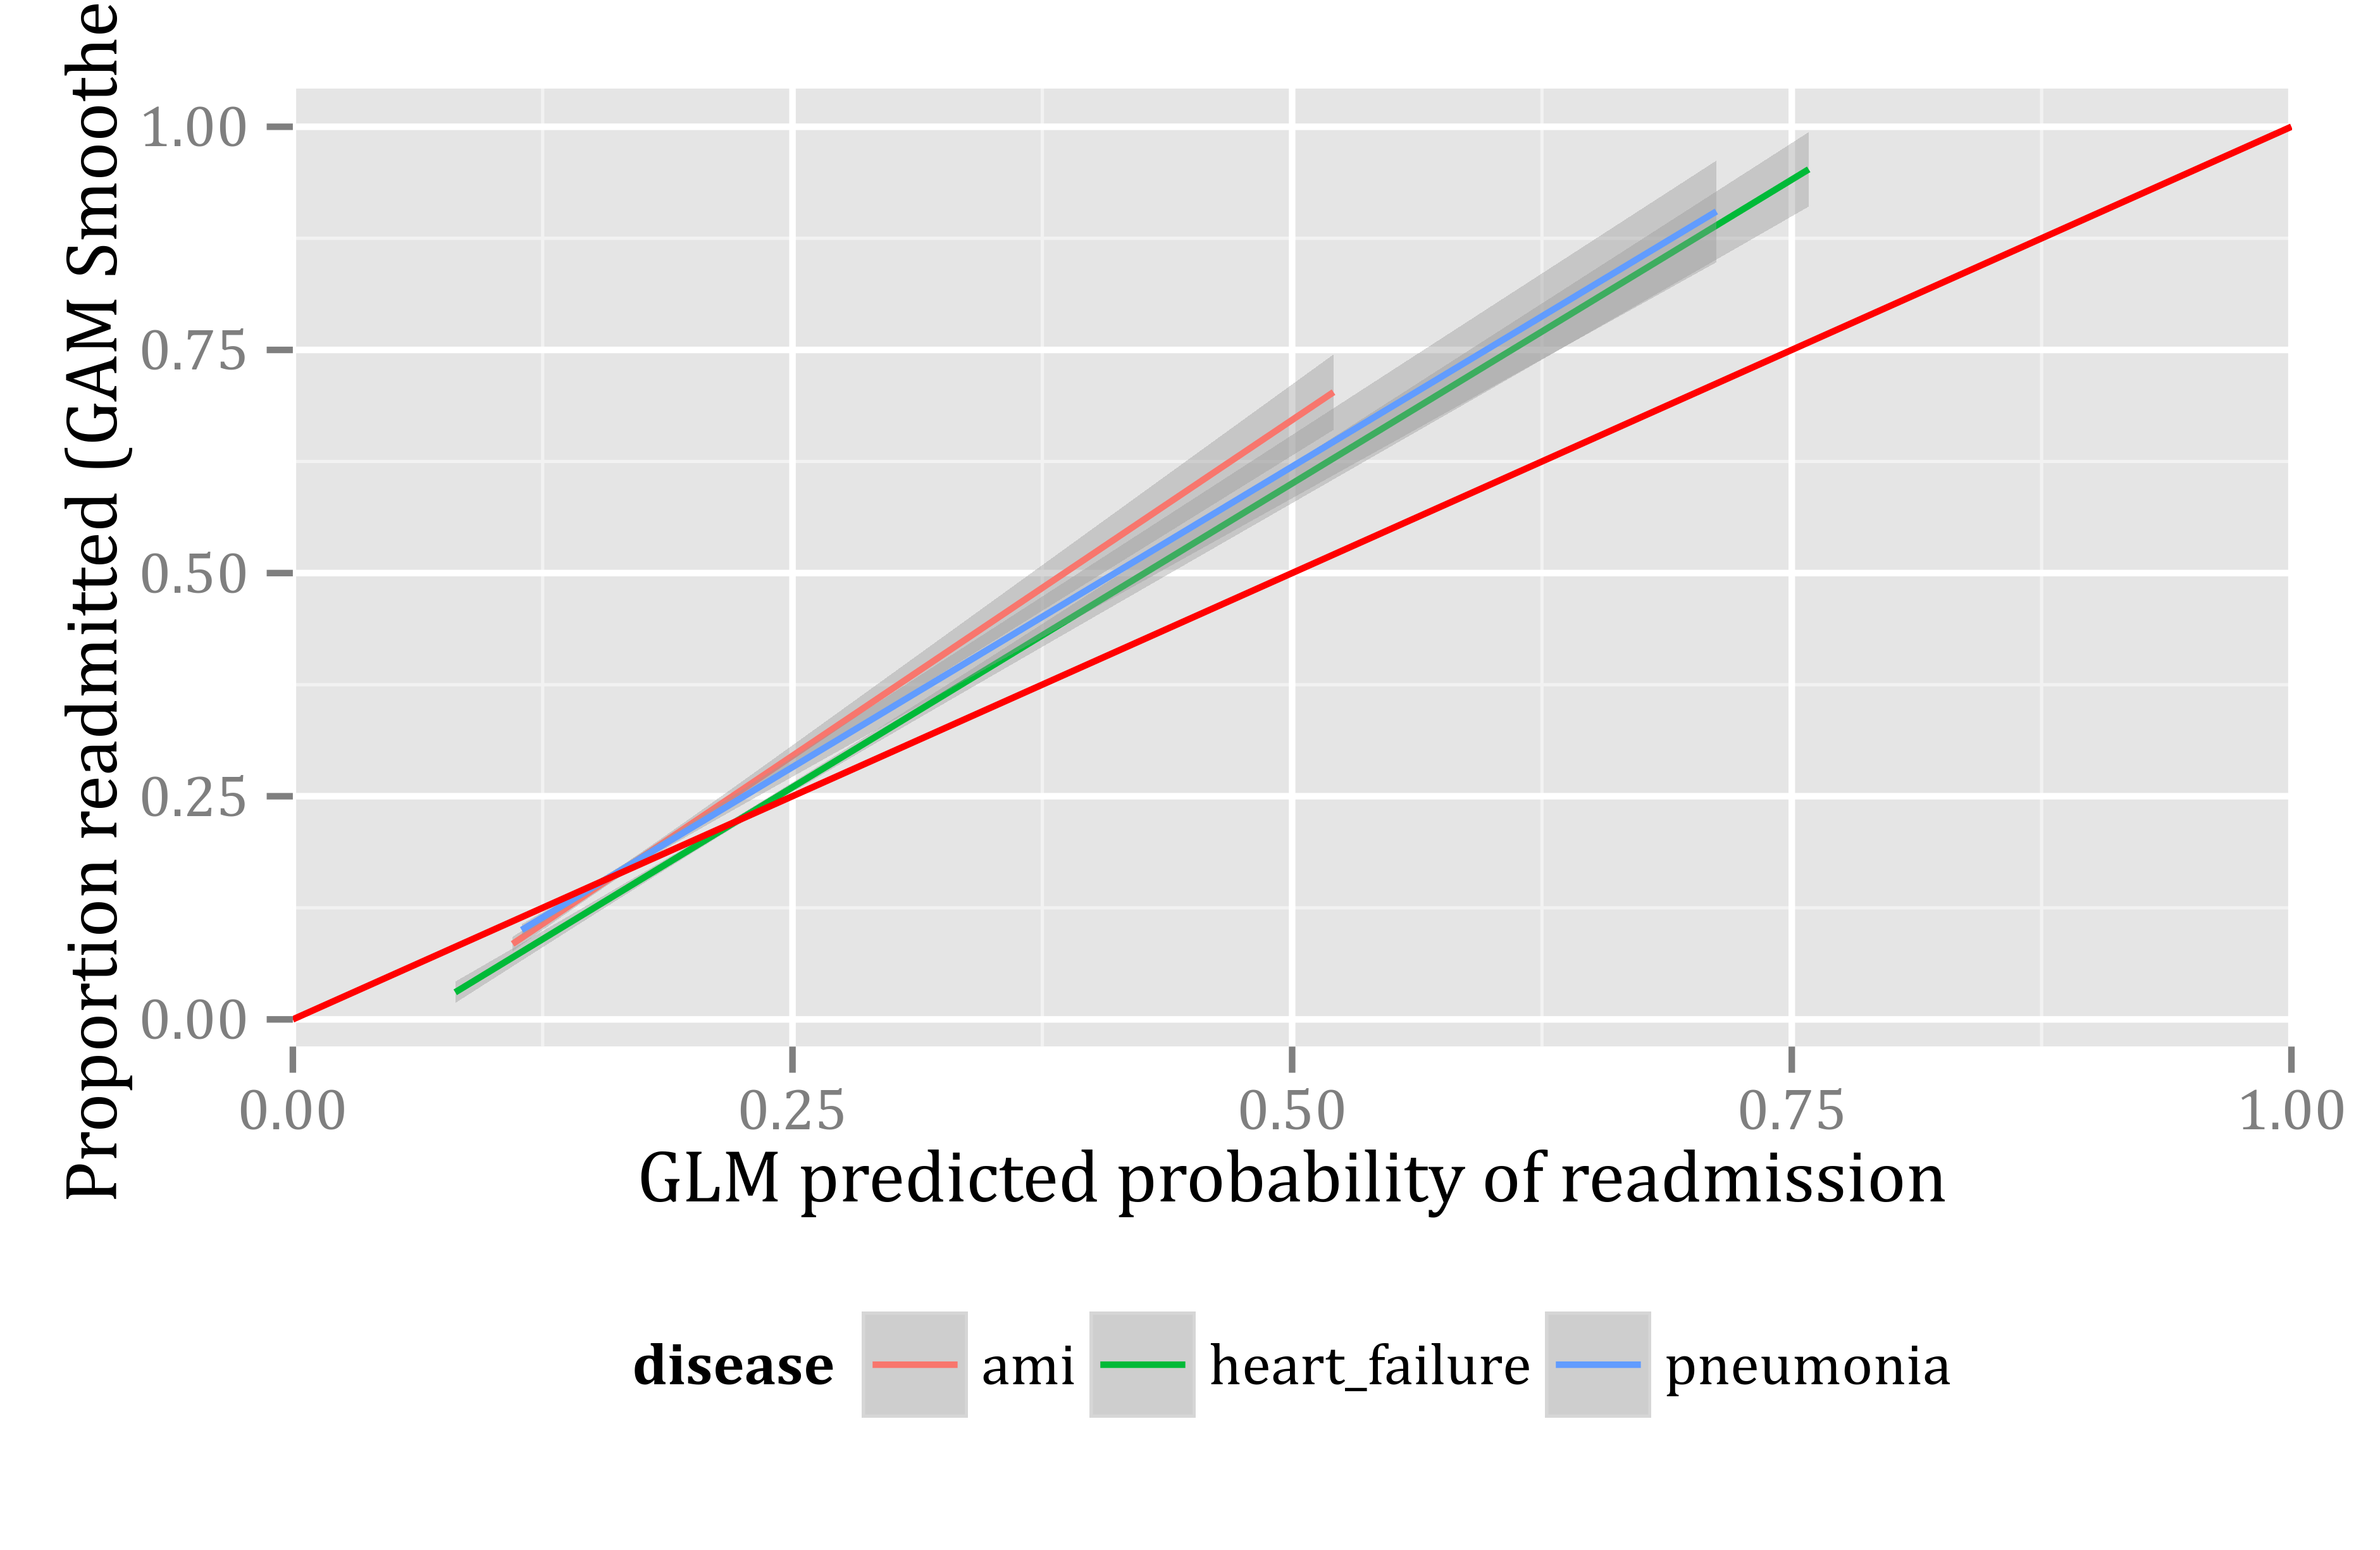
\includegraphics{../figures/glmnet_calibration.png}
%     \caption[Calibration for GLMnet model of hospital readmission.]
%       {Calibration for GLMnet model of hospital readmission. A descriptive sentence.}
%     \label{fig:error_rate_for_hospital_choice}
% \end{figure}

% What are the top 10 predictive variables for the hospitals by disease?
% \begin{figure}[H]
%     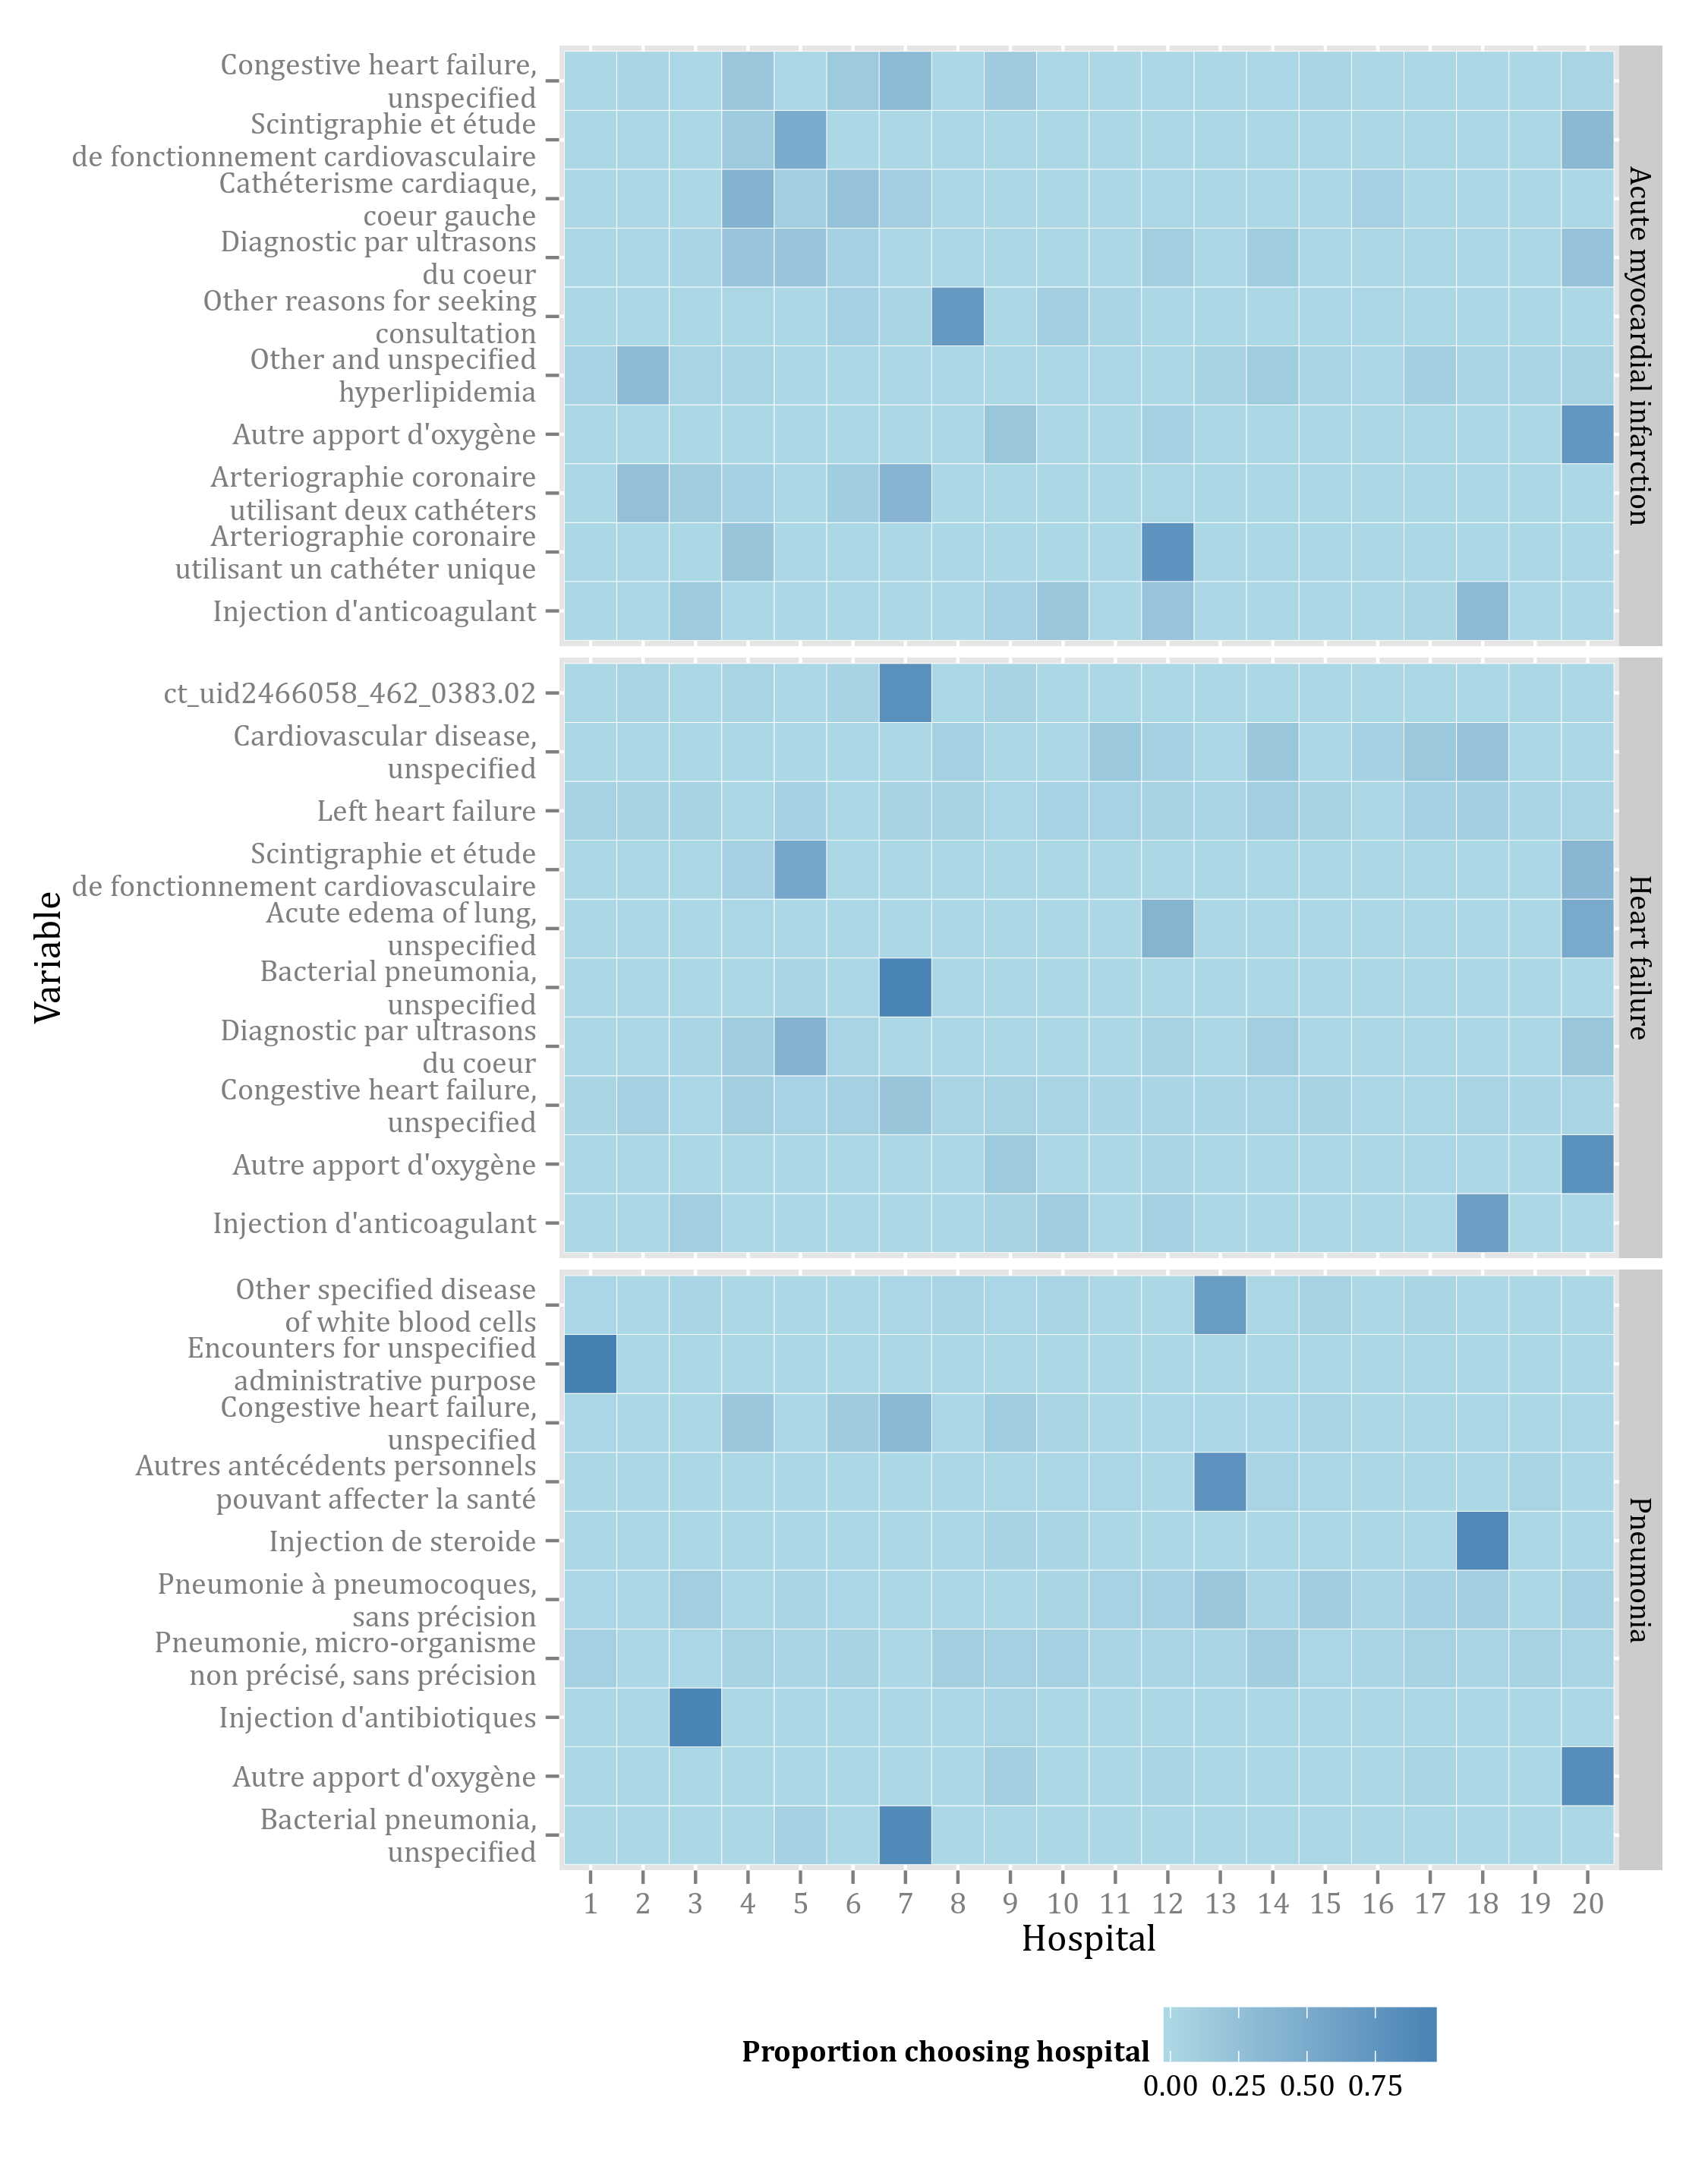
\includegraphics{../figures/top_10_variable_importance_and_hospital.png}
%     \caption[Error rate for random forest model of hospital choice.]
%       {10 most important variables for the G model, by disease. A descriptive sentence.}
%     \label{fig:top_10_variable_importance_and_hospital}
% \end{figure}

% How important are the different variables for each model by class?
\begin{figure}[H]
    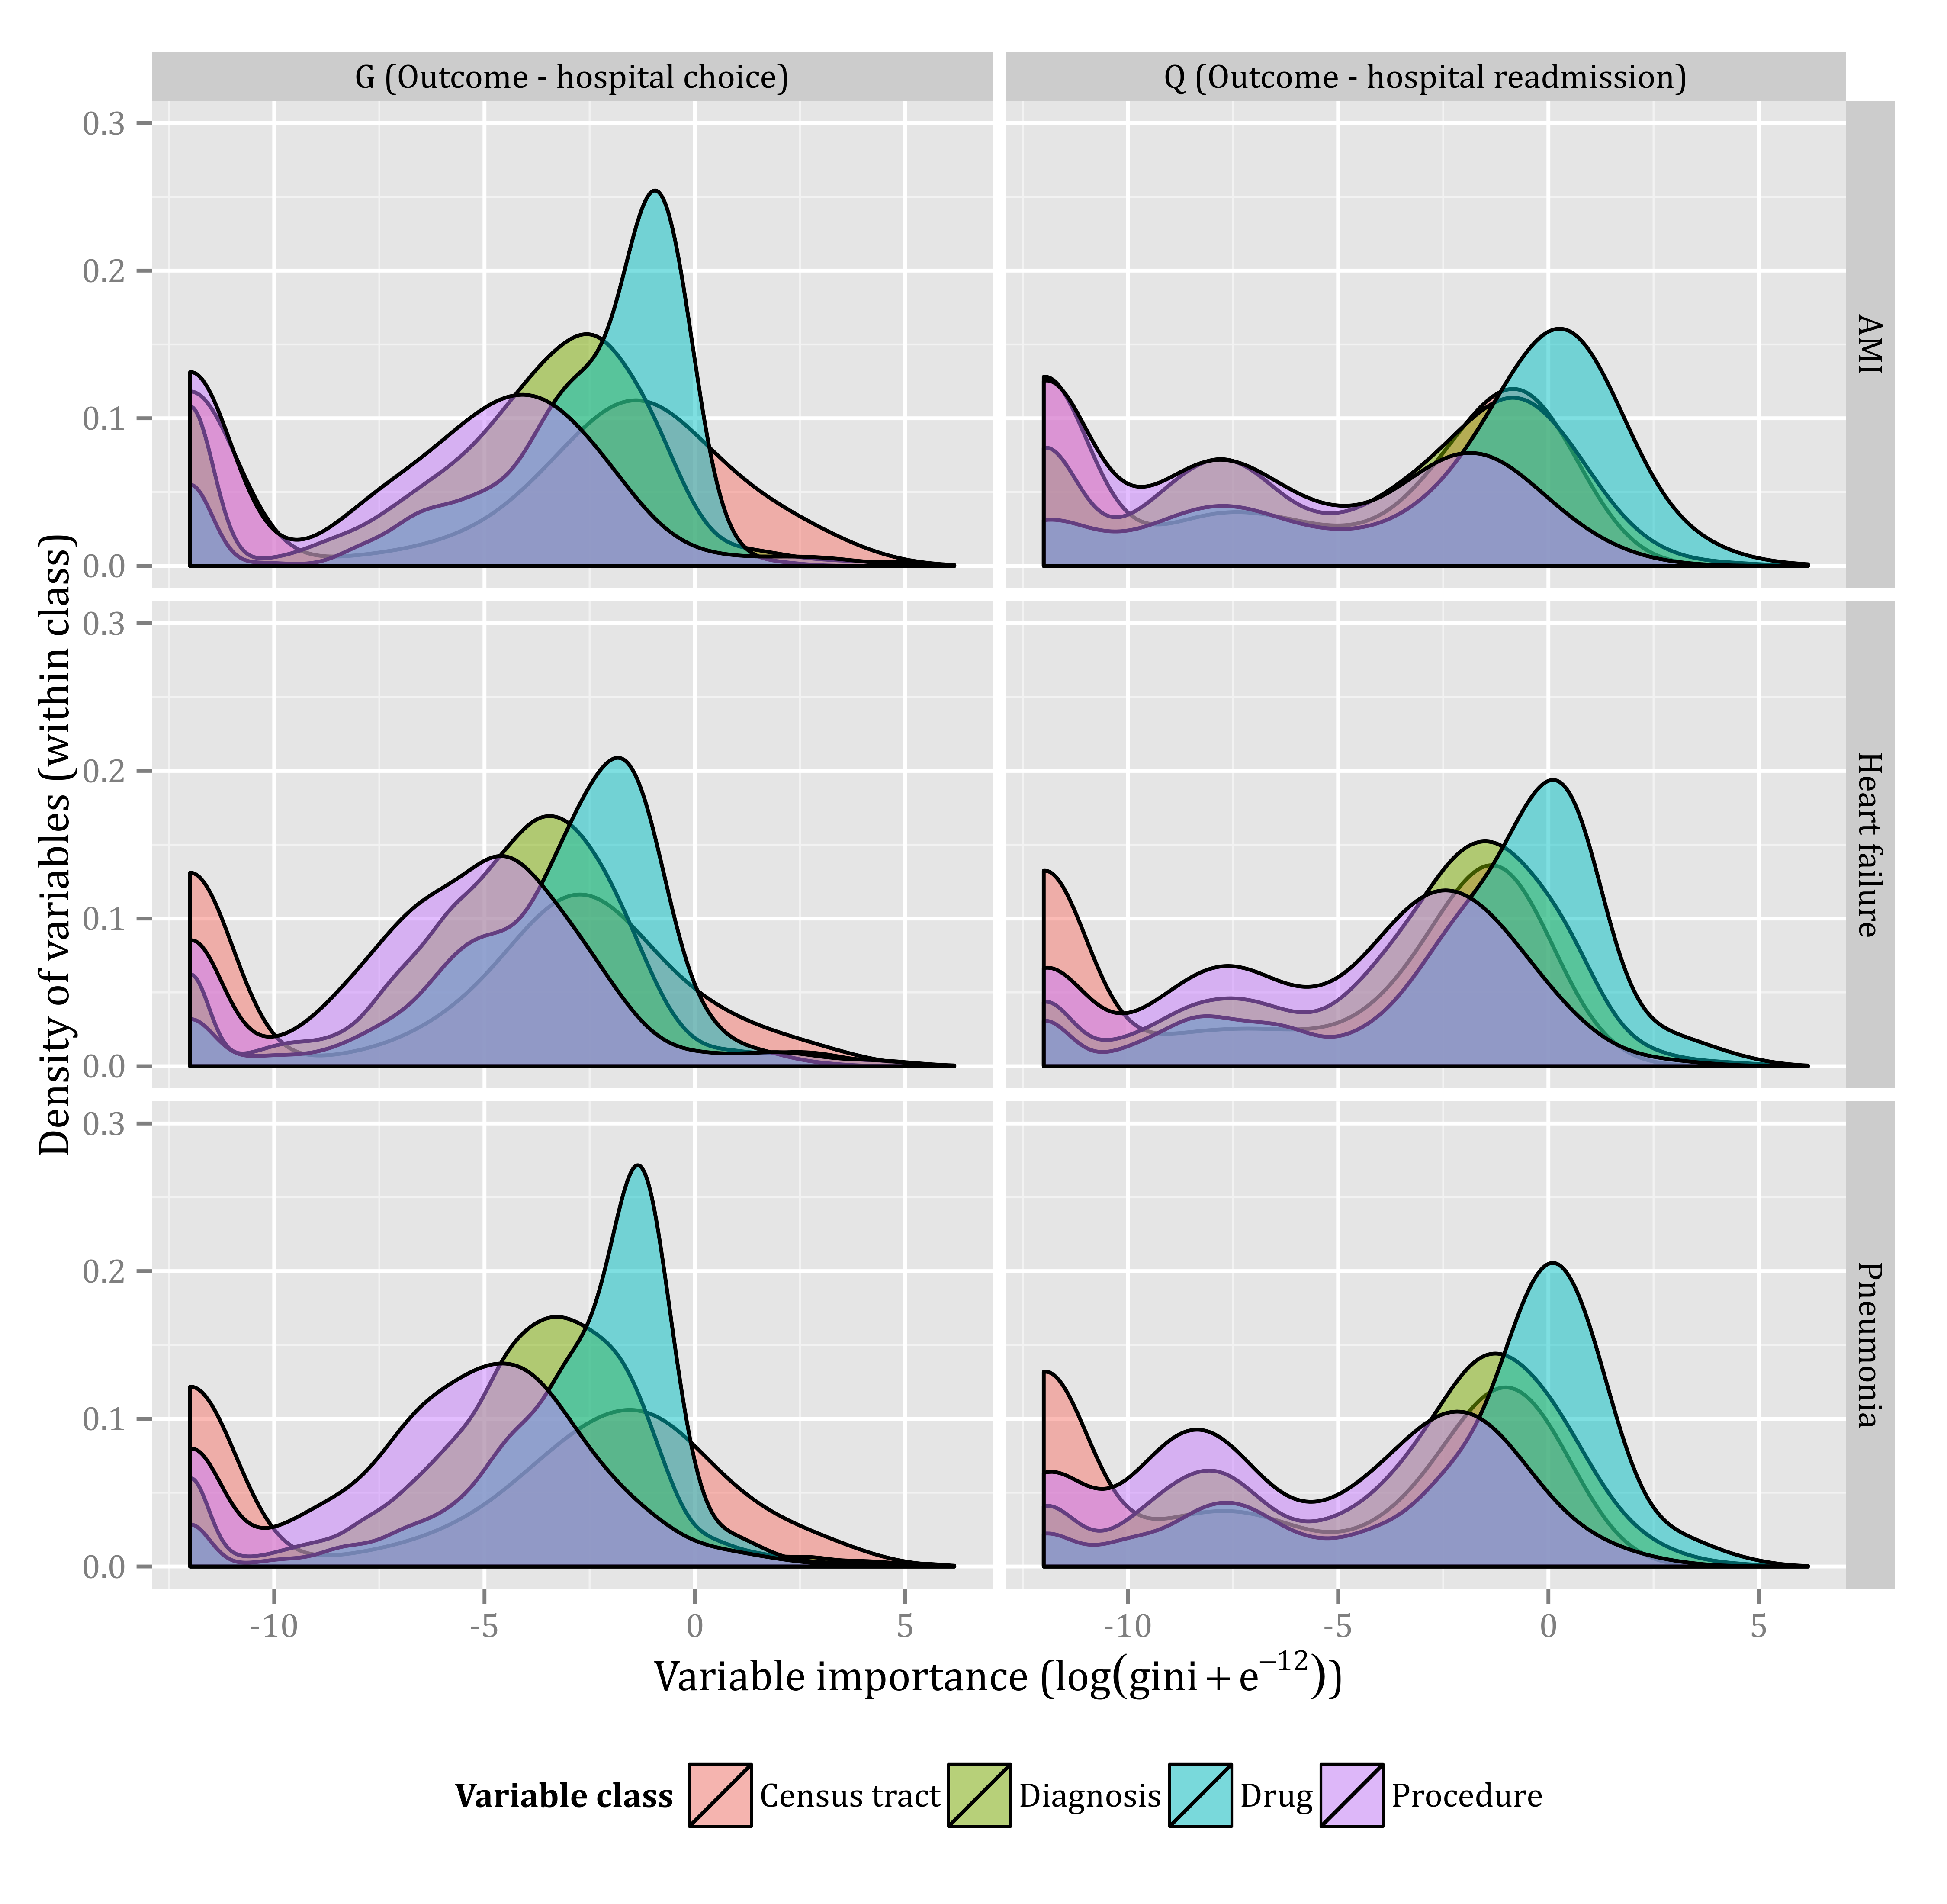
\includegraphics{../figures/variable_importance_by_model_and_class.png}
    \caption[Error rate for random forest model of hospital choice.]
      {Variable importance by model and variable class. A descriptive sentence.}
    \label{fig:variable_importance_by_model_and_class}
\end{figure}

% How does the glmnet model compare accuracy to the random forest model?
% What are the most important variables?

% Some tables.
\begin{landscape}

\setmainfont[Scale=1]{Cambria}
\linespread{1}

%latex.default(round(table, 2), file = "", cgroup = c("", "Length of stay (mean days)",     "", "Random Forest", "GLMnet"), n.cgroup = c(4, 3, 2, 3,     3), rowlabel = "Hospital", caption.loc = "bottom", caption = "Acute myocardial infarction (AMI).")%
\begin{table}[!tbp]
\begin{center}
\begin{tabular}{lrrrrcrrrcrrcrrrcrrr}
\hline\hline
\multicolumn{1}{l}{\bfseries Hospital}&\multicolumn{4}{c}{\bfseries }&\multicolumn{1}{c}{\bfseries }&\multicolumn{3}{c}{\bfseries Length of stay (mean days)}&\multicolumn{1}{c}{\bfseries }&\multicolumn{2}{c}{\bfseries }&\multicolumn{1}{c}{\bfseries }&\multicolumn{3}{c}{\bfseries Random Forest}&\multicolumn{1}{c}{\bfseries }&\multicolumn{3}{c}{\bfseries GLMnet}\tabularnewline
\cline{7-9} \cline{14-16} \cline{18-20}
\multicolumn{1}{l}{}&\multicolumn{1}{c}{Admitted}&\multicolumn{1}{c}{Died}&\multicolumn{1}{c}{(\%)}&\multicolumn{1}{c}{Discharged}&\multicolumn{1}{c}{}&\multicolumn{1}{c}{Admitted}&\multicolumn{1}{c}{Died}&\multicolumn{1}{c}{Discharged}&\multicolumn{1}{c}{}&\multicolumn{1}{c}{Readmitted}&\multicolumn{1}{c}{(\%)}&\multicolumn{1}{c}{}&\multicolumn{1}{c}{Q}&\multicolumn{1}{c}{ε}&\multicolumn{1}{c}{Q*}&\multicolumn{1}{c}{}&\multicolumn{1}{c}{Q}&\multicolumn{1}{c}{ε}&\multicolumn{1}{c}{Q*}\tabularnewline
\hline
1&$ 763$&$112$&$0.15$&$ 651$&&$15$&$10$&$16$&&$105$&$0.16$&&$0.16$&$ 0.00$&$0.16$&&$0.16$&$ 0.00$&$0.16$\tabularnewline
2&$1557$&$148$&$0.10$&$1409$&&$13$&$12$&$14$&&$191$&$0.14$&&$0.16$&$ 0.00$&$0.16$&&$0.16$&$ 0.00$&$0.16$\tabularnewline
3&$ 606$&$ 83$&$0.14$&$ 523$&&$14$&$12$&$14$&&$ 84$&$0.16$&&$0.16$&$ 0.00$&$0.16$&&$0.16$&$ 0.00$&$0.16$\tabularnewline
4&$1022$&$125$&$0.12$&$ 897$&&$11$&$ 7$&$12$&&$136$&$0.15$&&$0.16$&$ 0.00$&$0.16$&&$0.16$&$ 0.00$&$0.16$\tabularnewline
5&$ 729$&$150$&$0.21$&$ 579$&&$14$&$12$&$15$&&$ 98$&$0.17$&&$0.16$&$ 0.00$&$0.16$&&$0.16$&$ 0.00$&$0.16$\tabularnewline
6&$ 826$&$119$&$0.14$&$ 707$&&$11$&$ 8$&$12$&&$106$&$0.15$&&$0.16$&$ 0.00$&$0.16$&&$0.16$&$ 0.00$&$0.16$\tabularnewline
7&$1491$&$241$&$0.16$&$1250$&&$15$&$14$&$16$&&$216$&$0.17$&&$0.16$&$ 0.00$&$0.16$&&$0.16$&$ 0.00$&$0.16$\tabularnewline
8&$1270$&$198$&$0.16$&$1072$&&$14$&$12$&$15$&&$138$&$0.13$&&$0.16$&$-0.01$&$0.15$&&$0.16$&$-0.01$&$0.15$\tabularnewline
9&$ 780$&$152$&$0.19$&$ 628$&&$13$&$12$&$14$&&$130$&$0.21$&&$0.16$&$ 0.00$&$0.16$&&$0.16$&$ 0.00$&$0.16$\tabularnewline
10&$ 778$&$124$&$0.16$&$ 654$&&$13$&$ 9$&$14$&&$123$&$0.19$&&$0.16$&$ 0.00$&$0.16$&&$0.16$&$ 0.00$&$0.16$\tabularnewline
11&$ 705$&$125$&$0.18$&$ 580$&&$12$&$12$&$12$&&$ 97$&$0.17$&&$0.16$&$ 0.01$&$0.17$&&$0.16$&$ 0.01$&$0.17$\tabularnewline
12&$1284$&$266$&$0.21$&$1018$&&$15$&$14$&$15$&&$166$&$0.16$&&$0.16$&$ 0.00$&$0.16$&&$0.16$&$ 0.00$&$0.16$\tabularnewline
13&$ 739$&$ 86$&$0.12$&$ 653$&&$15$&$13$&$15$&&$110$&$0.17$&&$0.16$&$ 0.00$&$0.16$&&$0.16$&$ 0.00$&$0.16$\tabularnewline
14&$1307$&$184$&$0.14$&$1123$&&$12$&$ 8$&$13$&&$210$&$0.19$&&$0.16$&$ 0.00$&$0.16$&&$0.16$&$ 0.00$&$0.16$\tabularnewline
15&$1152$&$168$&$0.15$&$ 984$&&$16$&$14$&$17$&&$129$&$0.13$&&$0.16$&$-0.01$&$0.15$&&$0.16$&$-0.01$&$0.15$\tabularnewline
16&$ 408$&$ 70$&$0.17$&$ 338$&&$ 9$&$11$&$ 9$&&$ 43$&$0.13$&&$0.16$&$ 0.00$&$0.16$&&$0.16$&$ 0.00$&$0.16$\tabularnewline
17&$ 807$&$123$&$0.15$&$ 684$&&$11$&$15$&$11$&&$134$&$0.20$&&$0.16$&$ 0.00$&$0.16$&&$0.16$&$ 0.00$&$0.16$\tabularnewline
18&$ 894$&$144$&$0.16$&$ 750$&&$13$&$17$&$12$&&$116$&$0.15$&&$0.16$&$ 0.00$&$0.16$&&$0.16$&$ 0.00$&$0.16$\tabularnewline
19&$ 499$&$ 94$&$0.19$&$ 405$&&$ 9$&$12$&$ 8$&&$ 50$&$0.12$&&$0.16$&$-0.01$&$0.16$&&$0.16$&$-0.01$&$0.15$\tabularnewline
20&$1025$&$184$&$0.18$&$ 841$&&$13$&$ 9$&$14$&&$143$&$0.17$&&$0.16$&$ 0.00$&$0.16$&&$0.16$&$ 0.00$&$0.16$\tabularnewline
\hline
\end{tabular}

\caption{Acute myocardial infarction (AMI).\label{round}}\end{center}

\end{table}


%latex.default(round(table, 2), file = "", cgroup = c("", "Length of stay (mean days)",     "", "Random Forest", "GLMnet"), n.cgroup = c(4, 3, 2, 3,     3), rowlabel = "Hospital", caption.loc = "bottom", caption = "Heart failure")%
\begin{table}[!tbp]
\begin{center}
\begin{tabular}{lrrrrcrrrcrrcrrrcrrr}
\hline\hline
\multicolumn{1}{l}{\bfseries Hospital}&\multicolumn{4}{c}{\bfseries }&\multicolumn{1}{c}{\bfseries }&\multicolumn{3}{c}{\bfseries Length of stay (mean days)}&\multicolumn{1}{c}{\bfseries }&\multicolumn{2}{c}{\bfseries }&\multicolumn{1}{c}{\bfseries }&\multicolumn{3}{c}{\bfseries Random Forest}&\multicolumn{1}{c}{\bfseries }&\multicolumn{3}{c}{\bfseries GLMnet}\tabularnewline
\cline{7-9} \cline{14-16} \cline{18-20}
\multicolumn{1}{l}{}&\multicolumn{1}{c}{Admitted}&\multicolumn{1}{c}{Died}&\multicolumn{1}{c}{(\%)}&\multicolumn{1}{c}{Discharged}&\multicolumn{1}{c}{}&\multicolumn{1}{c}{Admitted}&\multicolumn{1}{c}{Died}&\multicolumn{1}{c}{Discharged}&\multicolumn{1}{c}{}&\multicolumn{1}{c}{Readmitted}&\multicolumn{1}{c}{(\%)}&\multicolumn{1}{c}{}&\multicolumn{1}{c}{Q}&\multicolumn{1}{c}{ε}&\multicolumn{1}{c}{Q*}&\multicolumn{1}{c}{}&\multicolumn{1}{c}{Q}&\multicolumn{1}{c}{ε}&\multicolumn{1}{c}{Q*}\tabularnewline
\hline
1&$1229$&$141$&$0.11$&$1088$&&$13$&$15$&$13$&&$248$&$0.23$&&$0.22$&$-0.02$&$0.21$&&$0.22$&$-0.02$&$0.21$\tabularnewline
2&$2071$&$166$&$0.08$&$1905$&&$13$&$19$&$12$&&$441$&$0.23$&&$0.22$&$ 0.00$&$0.22$&&$0.22$&$ 0.00$&$0.22$\tabularnewline
3&$1243$&$134$&$0.11$&$1109$&&$14$&$18$&$13$&&$285$&$0.26$&&$0.22$&$-0.01$&$0.21$&&$0.22$&$-0.01$&$0.21$\tabularnewline
4&$1076$&$122$&$0.11$&$ 954$&&$12$&$15$&$12$&&$214$&$0.22$&&$0.22$&$-0.01$&$0.22$&&$0.22$&$-0.01$&$0.22$\tabularnewline
5&$1550$&$181$&$0.12$&$1369$&&$12$&$17$&$11$&&$288$&$0.21$&&$0.22$&$-0.01$&$0.21$&&$0.22$&$-0.01$&$0.21$\tabularnewline
6&$ 827$&$107$&$0.13$&$ 720$&&$11$&$13$&$11$&&$128$&$0.18$&&$0.22$&$-0.02$&$0.21$&&$0.22$&$-0.02$&$0.21$\tabularnewline
7&$2917$&$386$&$0.13$&$2531$&&$13$&$17$&$12$&&$666$&$0.26$&&$0.22$&$ 0.00$&$0.22$&&$0.23$&$ 0.00$&$0.24$\tabularnewline
8&$1456$&$197$&$0.14$&$1259$&&$12$&$19$&$11$&&$232$&$0.18$&&$0.22$&$-0.02$&$0.21$&&$0.22$&$-0.02$&$0.21$\tabularnewline
9&$ 881$&$111$&$0.13$&$ 770$&&$13$&$21$&$12$&&$157$&$0.20$&&$0.22$&$ 0.00$&$0.22$&&$0.22$&$ 0.00$&$0.22$\tabularnewline
10&$1410$&$149$&$0.11$&$1261$&&$10$&$18$&$ 9$&&$311$&$0.25$&&$0.22$&$-0.01$&$0.22$&&$0.22$&$-0.01$&$0.22$\tabularnewline
11&$1297$&$153$&$0.12$&$1144$&&$17$&$24$&$16$&&$258$&$0.23$&&$0.22$&$-0.01$&$0.21$&&$0.22$&$-0.02$&$0.21$\tabularnewline
12&$1323$&$162$&$0.12$&$1161$&&$15$&$20$&$15$&&$192$&$0.17$&&$0.22$&$-0.01$&$0.22$&&$0.20$&$ 0.00$&$0.20$\tabularnewline
13&$1231$&$102$&$0.08$&$1129$&&$16$&$21$&$15$&&$262$&$0.23$&&$0.22$&$-0.01$&$0.22$&&$0.22$&$-0.01$&$0.21$\tabularnewline
14&$2110$&$234$&$0.11$&$1876$&&$11$&$15$&$11$&&$424$&$0.23$&&$0.22$&$-0.01$&$0.22$&&$0.22$&$-0.01$&$0.22$\tabularnewline
15&$1389$&$190$&$0.14$&$1199$&&$18$&$20$&$17$&&$203$&$0.17$&&$0.22$&$ 0.00$&$0.22$&&$0.22$&$ 0.00$&$0.22$\tabularnewline
16&$ 681$&$ 94$&$0.14$&$ 587$&&$11$&$15$&$10$&&$111$&$0.19$&&$0.22$&$-0.02$&$0.21$&&$0.22$&$-0.03$&$0.20$\tabularnewline
17&$1438$&$139$&$0.10$&$1299$&&$12$&$26$&$10$&&$328$&$0.25$&&$0.22$&$ 0.01$&$0.23$&&$0.22$&$ 0.01$&$0.23$\tabularnewline
18&$1984$&$212$&$0.11$&$1772$&&$14$&$24$&$13$&&$438$&$0.25$&&$0.22$&$-0.01$&$0.22$&&$0.22$&$-0.01$&$0.22$\tabularnewline
19&$ 932$&$ 99$&$0.11$&$ 833$&&$ 9$&$15$&$ 8$&&$163$&$0.20$&&$0.22$&$-0.01$&$0.21$&&$0.22$&$-0.02$&$0.21$\tabularnewline
20&$1048$&$167$&$0.16$&$ 881$&&$11$&$12$&$11$&&$171$&$0.19$&&$0.22$&$ 0.00$&$0.22$&&$0.22$&$ 0.00$&$0.22$\tabularnewline
\hline
\end{tabular}

\caption{Heart failure\label{round}}\end{center}

\end{table}


%latex.default(round(table, 2), file = "", cgroup = c("", "Length of stay (mean days)",     "", "Random Forest", "GLMnet"), n.cgroup = c(4, 3, 2, 3,     3), rowlabel = "Hospital", caption.loc = "bottom", caption = "Pneumonia")%
\begin{table}[!tbp]
\begin{center}
\begin{tabular}{lrrrrcrrrcrrcrrrcrrr}
\hline\hline
\multicolumn{1}{l}{\bfseries Hospital}&\multicolumn{4}{c}{\bfseries }&\multicolumn{1}{c}{\bfseries }&\multicolumn{3}{c}{\bfseries Length of stay (mean days)}&\multicolumn{1}{c}{\bfseries }&\multicolumn{2}{c}{\bfseries }&\multicolumn{1}{c}{\bfseries }&\multicolumn{3}{c}{\bfseries Random Forest}&\multicolumn{1}{c}{\bfseries }&\multicolumn{3}{c}{\bfseries GLMnet}\tabularnewline
\cline{7-9} \cline{14-16} \cline{18-20}
\multicolumn{1}{l}{}&\multicolumn{1}{c}{Admitted}&\multicolumn{1}{c}{Died}&\multicolumn{1}{c}{(\%)}&\multicolumn{1}{c}{Discharged}&\multicolumn{1}{c}{}&\multicolumn{1}{c}{Admitted}&\multicolumn{1}{c}{Died}&\multicolumn{1}{c}{Discharged}&\multicolumn{1}{c}{}&\multicolumn{1}{c}{Readmitted}&\multicolumn{1}{c}{(\%)}&\multicolumn{1}{c}{}&\multicolumn{1}{c}{Q}&\multicolumn{1}{c}{ε}&\multicolumn{1}{c}{Q*}&\multicolumn{1}{c}{}&\multicolumn{1}{c}{Q}&\multicolumn{1}{c}{ε}&\multicolumn{1}{c}{Q*}\tabularnewline
\hline
1&$1184$&$176$&$0.15$&$1008$&&$13$&$14$&$13$&&$159$&$0.16$&&$0.16$&$-0.01$&$0.15$&&$0.16$&$-0.01$&$0.15$\tabularnewline
2&$ 199$&$ 11$&$0.06$&$ 188$&&$13$&$15$&$12$&&$ 31$&$0.16$&&$0.16$&$-0.01$&$0.15$&&$0.16$&$-0.01$&$0.15$\tabularnewline
3&$1085$&$132$&$0.12$&$ 953$&&$13$&$15$&$13$&&$160$&$0.17$&&$0.16$&$ 0.00$&$0.16$&&$0.16$&$ 0.00$&$0.15$\tabularnewline
4&$ 863$&$ 91$&$0.11$&$ 772$&&$13$&$14$&$12$&&$113$&$0.15$&&$0.16$&$ 0.00$&$0.16$&&$0.16$&$ 0.00$&$0.16$\tabularnewline
5&$ 923$&$147$&$0.16$&$ 776$&&$11$&$13$&$11$&&$143$&$0.18$&&$0.16$&$ 0.00$&$0.16$&&$0.16$&$ 0.00$&$0.16$\tabularnewline
6&$ 788$&$136$&$0.17$&$ 652$&&$12$&$15$&$11$&&$ 89$&$0.14$&&$0.16$&$ 0.00$&$0.15$&&$0.16$&$ 0.00$&$0.15$\tabularnewline
7&$2194$&$228$&$0.10$&$1966$&&$15$&$16$&$14$&&$328$&$0.17$&&$0.16$&$ 0.00$&$0.16$&&$0.16$&$ 0.00$&$0.16$\tabularnewline
8&$1485$&$243$&$0.16$&$1242$&&$11$&$14$&$11$&&$173$&$0.14$&&$0.16$&$-0.01$&$0.15$&&$0.16$&$-0.01$&$0.15$\tabularnewline
9&$ 990$&$166$&$0.17$&$ 824$&&$15$&$16$&$15$&&$158$&$0.19$&&$0.16$&$ 0.00$&$0.16$&&$0.16$&$ 0.00$&$0.16$\tabularnewline
10&$1214$&$139$&$0.11$&$1075$&&$11$&$14$&$11$&&$181$&$0.17$&&$0.16$&$ 0.00$&$0.16$&&$0.16$&$ 0.00$&$0.15$\tabularnewline
11&$ 892$&$147$&$0.16$&$ 745$&&$14$&$20$&$14$&&$119$&$0.16$&&$0.16$&$ 0.00$&$0.16$&&$0.16$&$ 0.00$&$0.16$\tabularnewline
12&$1102$&$185$&$0.17$&$ 917$&&$14$&$13$&$15$&&$ 91$&$0.10$&&$0.16$&$-0.03$&$0.13$&&$0.15$&$-0.04$&$0.12$\tabularnewline
13&$1914$&$204$&$0.11$&$1710$&&$14$&$14$&$14$&&$325$&$0.19$&&$0.16$&$ 0.00$&$0.16$&&$0.16$&$ 0.00$&$0.16$\tabularnewline
14&$1980$&$278$&$0.14$&$1702$&&$11$&$12$&$11$&&$263$&$0.15$&&$0.16$&$-0.01$&$0.15$&&$0.16$&$-0.01$&$0.15$\tabularnewline
15&$1365$&$179$&$0.13$&$1186$&&$11$&$14$&$11$&&$163$&$0.14$&&$0.16$&$ 0.00$&$0.15$&&$0.16$&$-0.01$&$0.15$\tabularnewline
16&$ 541$&$ 77$&$0.14$&$ 464$&&$13$&$17$&$12$&&$ 46$&$0.10$&&$0.16$&$-0.01$&$0.15$&&$0.16$&$-0.01$&$0.15$\tabularnewline
17&$1338$&$163$&$0.12$&$1175$&&$10$&$18$&$ 9$&&$193$&$0.16$&&$0.16$&$ 0.01$&$0.16$&&$0.16$&$ 0.00$&$0.16$\tabularnewline
18&$1356$&$168$&$0.12$&$1188$&&$15$&$22$&$14$&&$200$&$0.17$&&$0.16$&$ 0.01$&$0.16$&&$0.16$&$ 0.00$&$0.16$\tabularnewline
19&$1020$&$123$&$0.12$&$ 897$&&$10$&$19$&$ 9$&&$122$&$0.14$&&$0.16$&$-0.02$&$0.14$&&$0.16$&$-0.02$&$0.14$\tabularnewline
20&$1152$&$171$&$0.15$&$ 981$&&$15$&$16$&$14$&&$126$&$0.13$&&$0.16$&$ 0.00$&$0.16$&&$0.16$&$ 0.00$&$0.15$\tabularnewline
\hline
\end{tabular}

\caption{Pneumonia\label{round}}\end{center}

\end{table}


\setmainfont[Scale=1.25]{Cambria}
\linespread{1.25}


\end{landscape}
\section{Discussion}
% The introduction
In this study, we estimated marginal risk of 30-day readmission adjusted for patient readmission risk in twenty Montreal hospitals, and found that the marginal risk differences were not as strong as the crudely estimated readmission risk suggested. 

In this study, we estimated the marginal risk of 30-day readmission and the mean time-to-readmission with machine learning techniques (random forest) and doubly-robust parameter estimation (TMLE) in twenty hospitals in Montreal.

% On the preventability of readmissions.
Several readmission risk models have been criticized on the basis that they failed to distinguish preventable readmissions from readmissions due to chance alone. Despite evidence that clincians cannot reliably distinguish preventable and non-preventable readmissions, pairs of diagnosis codes have been developed that are "potentially preventable". For example, following a hospitalization for surgery, a readmission for infection would be considered preventable, but a readmission for trauma would not.

We did not atempt to measure whether \emph{individual} readmissions were preventable, we instead opted to place readmissions within a counterfactual framework, and only identify the difference in readmission risk between hospitals, after controlling for differences in case-mix. 

% How does this relate to the counterfactual statement?
The counterfactual model clarifies the study question: What is the difference in the proportion with an emergency readmission within 30 days if all patients had attended Hospital A vs Hospital B? The notion of a "preventable" readmission is implicit; if a patient would have been readmitted if treated at another hospital, then the readmission was preventable. Since we cannot directly observe the desired proportions, we estimate it by attempting to recreate exchangeability (control for confounding) among the populations that visited different hospitals.

% No mediators.
Following other hospital readmission work, we did not include hospital length of stay as a risk factor for readmission. Although we have strong reason to believe that the length of stay may affect readmission risk (and varies between hospitals), it acts as a mediator between hospital care and readmission; if we included it in our models, we risk biasing our estimate of the hospital's effect on readmission. 

However, unlike many other hospital readmission studies, we also excluded all diagnoses and procedures that occurred during the hospital admission, because these covariates were also effectively mediators between hospital care and readmission. For example, hospital-acquired infections are one source of preventable readmissions; if we controlled for diagnosis codes indicating hospital-acquired infections, we would attenuate the effect that the hospital care was having on readmissions.

% Competing risks.
The major competing risk for hospital readmission is death, but others include moving outside the study area, or admission to a hospital for a non-emergency reason. If patients died within 30 days of discharge more often at one hospital than another, we could have biased our estimate of readmission risk.

% A selection bias.
Similarly, if patients died during the hospitalization more often at some hospitals than others, it could have created a selection bias in which hospitals with better care were discharging sicker (but still living) patients, who would be more likely to be readmitted. 

% 30-day problem
Finally, there is no special significance of 30 days in readmission, except for the fact that it is (recently) widely used as a cutoff. In future analyses, we plan to study the effect of hospital care on the time-to-readmission, to avoid any arbitrary cutoff times.   

% Readmission isn't always a bad thing. Maybe the probability of admission has changed.
Differing \emph{admission} practices can strongly affect the rates of readmission. Since most patients (x\% in this cohort) return to the same hospital after readmission, if a hospital is more likely to admit patients than others, it will have a higher readmission rate. In some cases, like a major trauma, admission is certain, and in other cases, like a mild infection, admission is very improbable, but in most cases, there is some uncertainty in how patients are admitted. In future work, we plan to study the effect of the probability of admission on readmission.

% The influenza cohort.
Entry to our cohort was dependent on having one diagnosis of a respiratory illness in an inpatient or outpatient setting. 


% Differential misclassification due to coding practices.

% We had a large cohort from all socioeconomic classes. We did not have to restrict to a single network in a city. The same covariates were measured across all hospitals. We could track if they went to "any" hospital in the province, which is expected to be the vast majority of visits.

% We could have adjusted for the problem that a patient may be measured multiple times. In some sense, this could be considered a multiple measurement problem. But, the strata are going to be very small, and there will be many of them; the effect on variance may be very small, and the computation very difficult. It is also not exactly clear how you would do this.
 
% The absolute risk difference is low, leading to a low marginal difference in the number readmitted between hospitals. Consider, however, that in all exposure/outcome analyses where the outcome is rare, and the exposure relatively balanced, the expected absolute difference will likely be small. 

% While it was totally possible to use SuperLearner (an ensemble learning technique), it was too computationally expensive; random forest is just one of the methods used in SuperLearner, and it was already very computationally expensive on these data.

% Calibration
Calibration of the random forest vote proportions in the Q model strongly affected estimates of our parameter of interest in the Q* update step. Other articles using non-parametric techniques typically combined them with other models in an ensemble learner (in particular SuperLearner has been often used with TMLE). The final step in the ensemble learner is to combine all the probability estimates in parametric model, which would effectively calibrate the probabilities. When a single, non-parametric technique is used, an additional, seperate calibration step is necessary to convert the ranking scores into a probability estimate.

\printbibliography

\end{document}
